% \chapter{Dynamics in the thermodynamic limit}
\newpage
\section[Detuned driving]{Analysis for the detuned driving}\label{sec:detuned_analysis}
After I examined the system in resonance with the driving laser, it is interesting to see, if the stability of the system remains, when a detuning is introduced. As the presence of a small detuning can not be completely avoided in reality, it is important to examine if the previously found properties withstand the onset of detuning, and are thus actually observable.\\
For the non-resonant driving $x=0$ is no stationary solution anymore, on the contrary $x$ and $y$ are coupled by the detuning in an oscillatory way. One can wonder, if this additional oscillation inducing term can effect the system in a way that the oscillations do not die out. In fact this is true. In this section I will show the rise of time crystal regimes and dedicate the section to two properties of the system, that I find most interesting. On the one hand subregions are found, where more than one limit cycle exists for the same parameter configuration and hence multistability arises. Additionally the division of the dynamics into a region of stationary and time crystal solutions, will be linked to synchronization behavior. The start of the analysis will again constitute the search for stable fixed points.


\subsection[stability in general]{Stability analysis of the fixed points}\label{sec:stab_3D}
The procedure by which the number of fixed points is determined as well as their stability is the same as previously. Because of the more complex structure of the equations of motion with detuning present the analysis will be performed numerically.\\
In this context the following system of equations is solved for stationary $m_x$- and $m_y$-values
\begin{align*}
    -\Gamma\delta\,m_y-\Gamma\,(\gamma+\Gamma-\kappa)\,m_x-2\,\kappa^2\,m_x\,( m_x^2+ m_y^2)+2\,\kappa\omega\,m_xm_y  &=0\\\\
    \Gamma\delta\,m_x-\omega\Gamma-\Gamma\,(\gamma+\Gamma-\kappa)\,m_y-2\,\omega^2\,m_y&\\
    -2\,\kappa^2\,m_y\,( m_x^2+ m_y^2)+2\,\kappa\omega\,(m_x^2+2\,m_y^2)  &=0\quad.
\end{align*}
% After multiplying the first equation by $m_y$ and the second by $m_x$, the two equations can be subtracted from each other.
% \begin{align*}
%     -\Gamma\delta\,(m_x^2+m_y^2)+\Gamma\omega\,m_x+2\,\omega^2\,m_xm_y-2\,\kappa\omega\,m_x\,(m_x^2+m_y^2)
% \end{align*}
% By solving this quadratic equation for $m_y$ analytically and plugging the result into the second equation, one has two find a root of a one variable function, which is computationally less expensive than determining the roots of the two dimensional problem. For the pursuit of this procedure I divided the x-axis into a grid and searched between the gridpoints for roots in order to find all of the fixed points.\\
% In critical regions, where this procedure did not work well, I created a 2D grid and solved the two dimensional problem.\\\\
As a result of the numerical calculation one finds, that there again exist two regions, one in which there is one fixed point and one in which three fixed points are present. The $\delta=0$ case is expanded continuously.
% \begin{align*}
%     m_{y,12}(m_x)=\frac{1}{\Gamma\delta+2\,\kappa\omega\,m_x}\,\left( \omega^2\,m_x\pm \sqrt{\omega^4\,m_x^2-(\Gamma\delta+2\,\kappa\omega\,m_x)\,[(\Gamma\delta+2\,\kappa\omega\,m_x)\,m_x^2-\Gamma\omega\,m_x]} \right)
% \end{align*}
\begin{figure}[H]
    % \vspace*{-1cm}
    \hspace*{-1.2cm}
    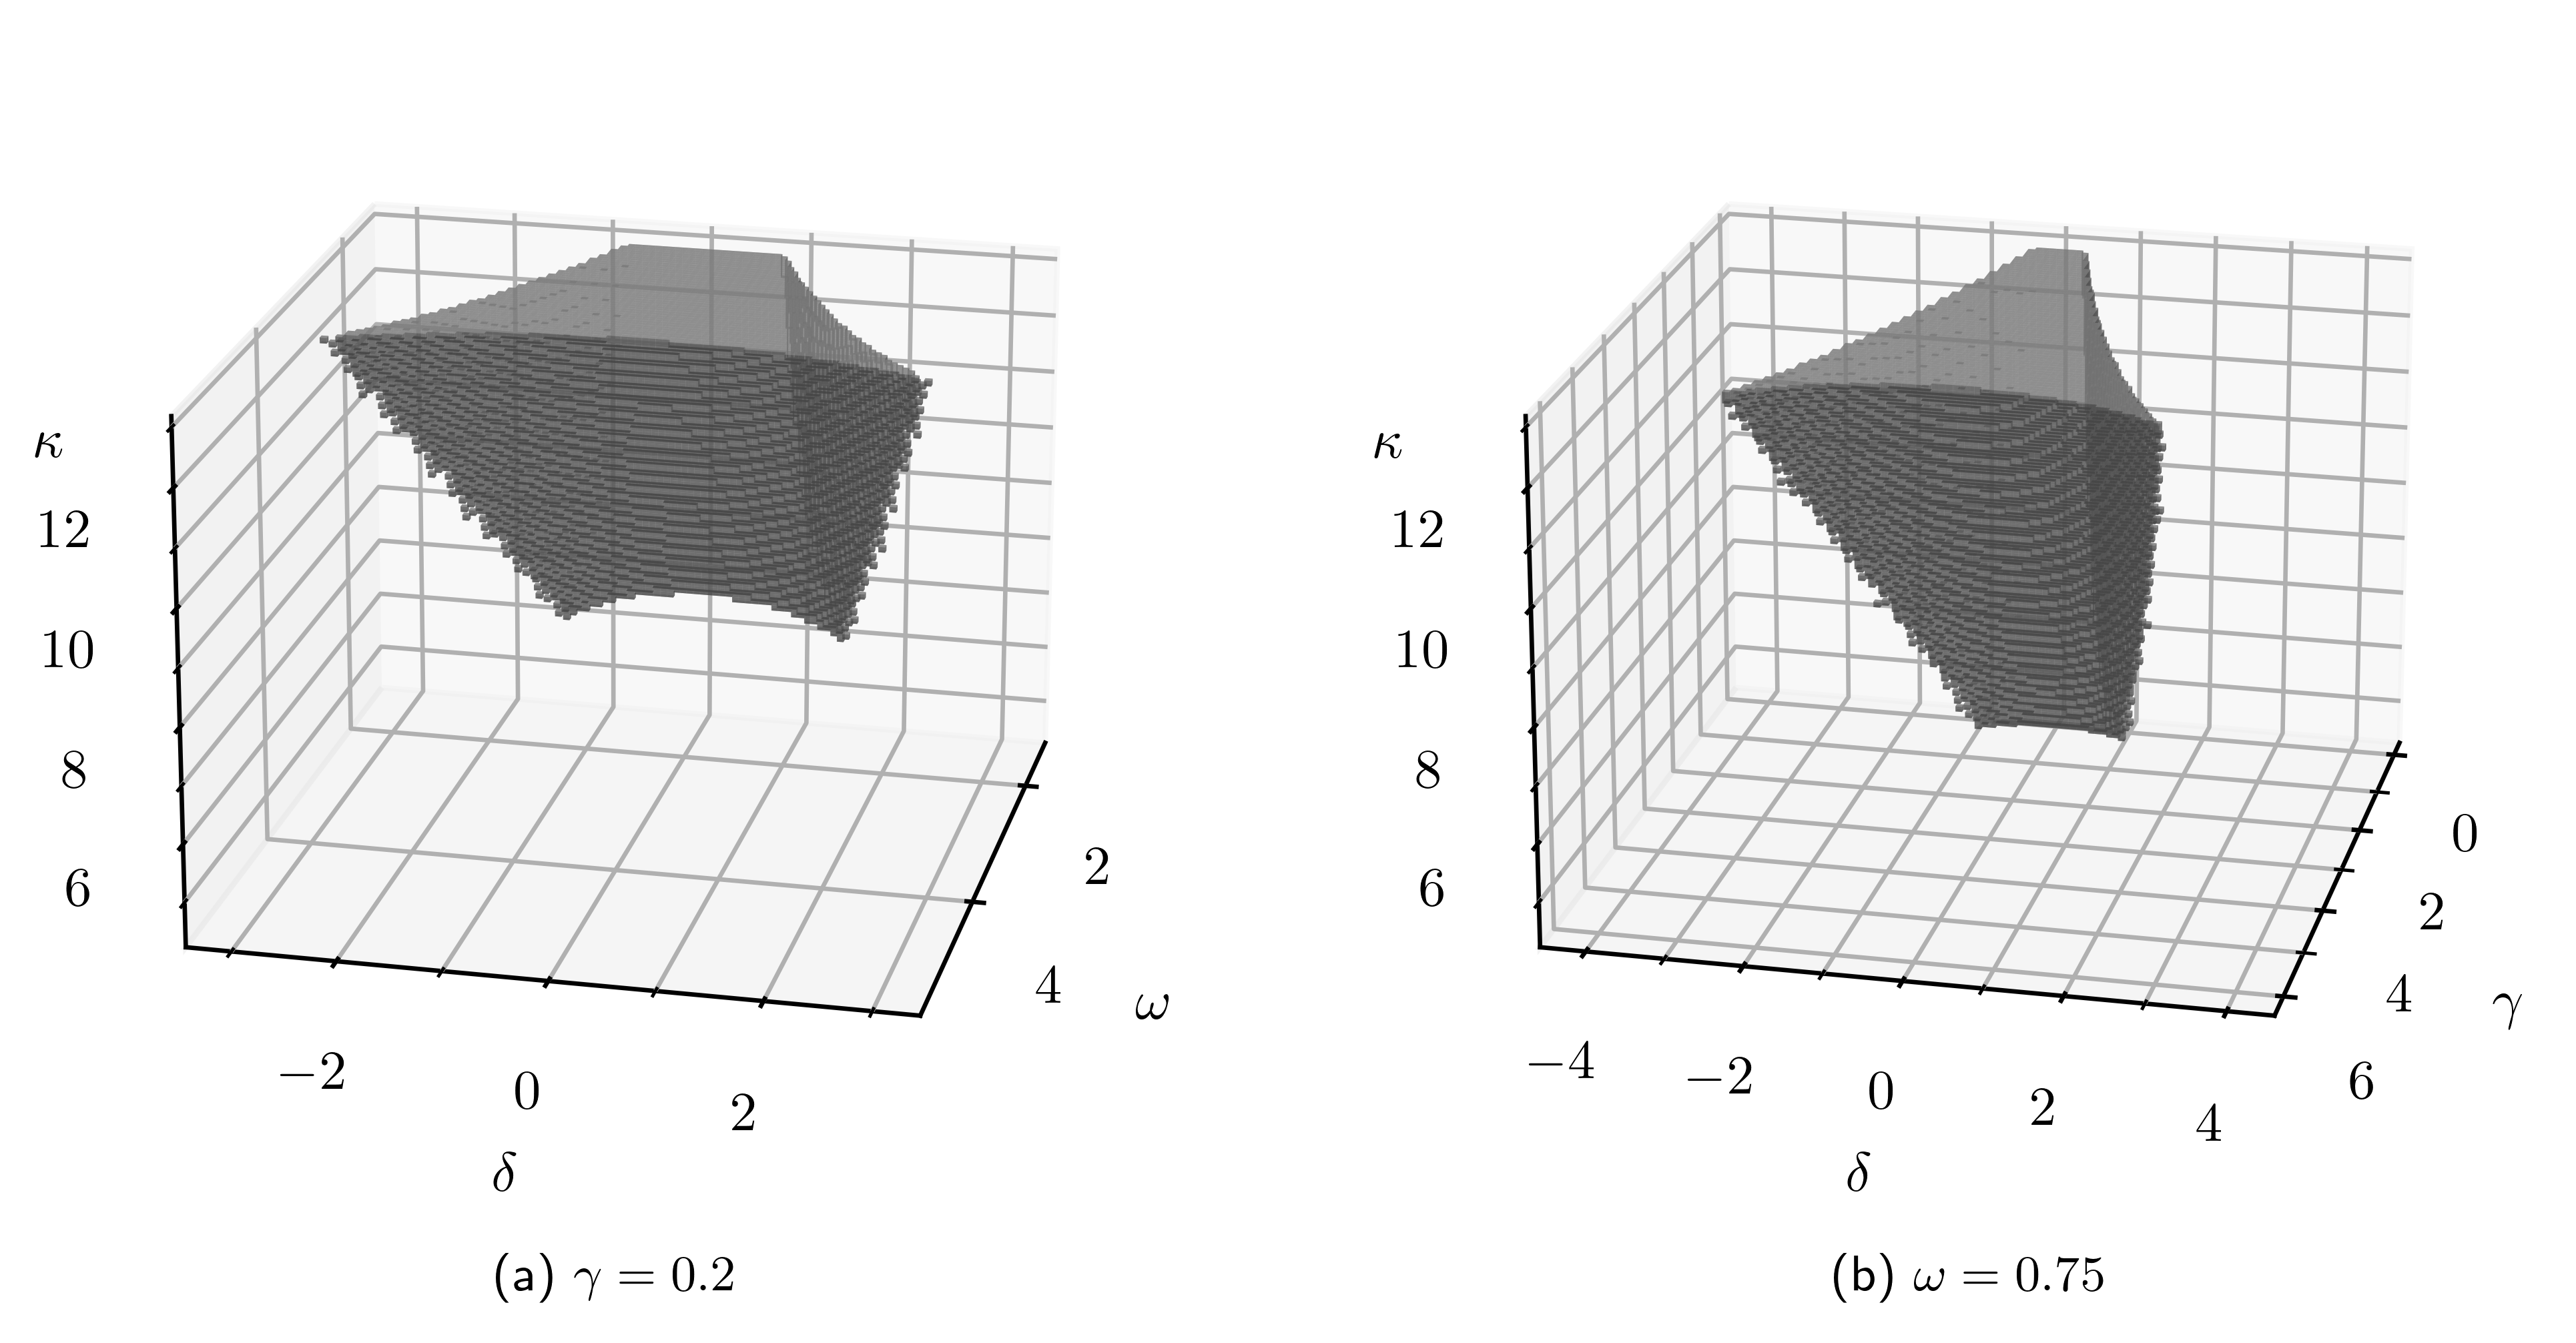
\includegraphics{pictures/numb_of_fixp_stab3d_gw.png}
    \caption{The gray filled region has 3 fixed points, whereas the rest of the shown parameter space has 1 fixed point. In the left graph $\gamma$ is held on $0.2$, where in the right graph $omega$ is fixed to $0.75$. The two parameters $\omega$ and $\gamma$ shape the regions of different numbers of fixedpoint similarly.}%Shown in the bottom row are different projectin views. They do not show cuts through parameter space, but projections of one parameter dimension onto the other two. I find this gives a better impression of the shape of the area with three stationary solutions.}
    \label{fig:numb_of_fixp_3D}
\end{figure}
The stability of the stationary solutions is also determined analogously to the zero detuning case. The equations of motion are linearized in the fixed points and the sign of the eigenvalues of the linearization is evaluated. The findings of this analysis draw a consistent picture with the one found for $\delta=0$, as shown in \figref{fig:stability_of_solutions}. Stable stationary solutions exist and complement the zero detuning case. But contrary to this case, here also regions, where no stable fixed points exist. Where no stable stationary solutions are found, more complicated behavior is expected, as for example limit cycles.
\begin{figure}[H]
    % \vspace*{-1cm}
    % \centering
    \hspace*{-1.2cm}
    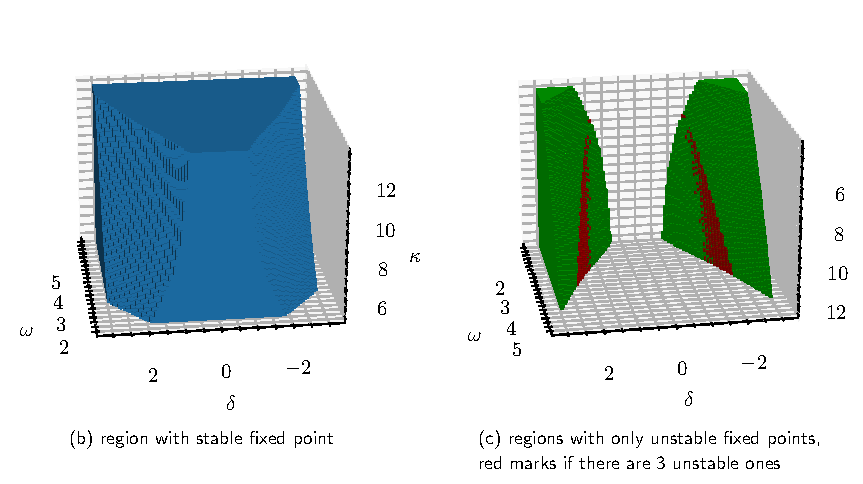
\includegraphics{pictures/stability_regions_2plots.pdf}
    \caption{Stability of the stationary points. The blue filled area has at least one stable fixed point, whereas in the green filled region there is no stable fixed point at all. One can also find a regime, in which there are three fixed points, but all of them are unstable. This area is marked red. Pumping and dephasing are set to $\Gamma=1$ and $\gamma=0.2$.}
    \label{fig:stability_of_solutions}
\end{figure}

\begin{figure}[H]
    \vspace*{-0.3cm}
    % \hspace*{-1.2cm}
    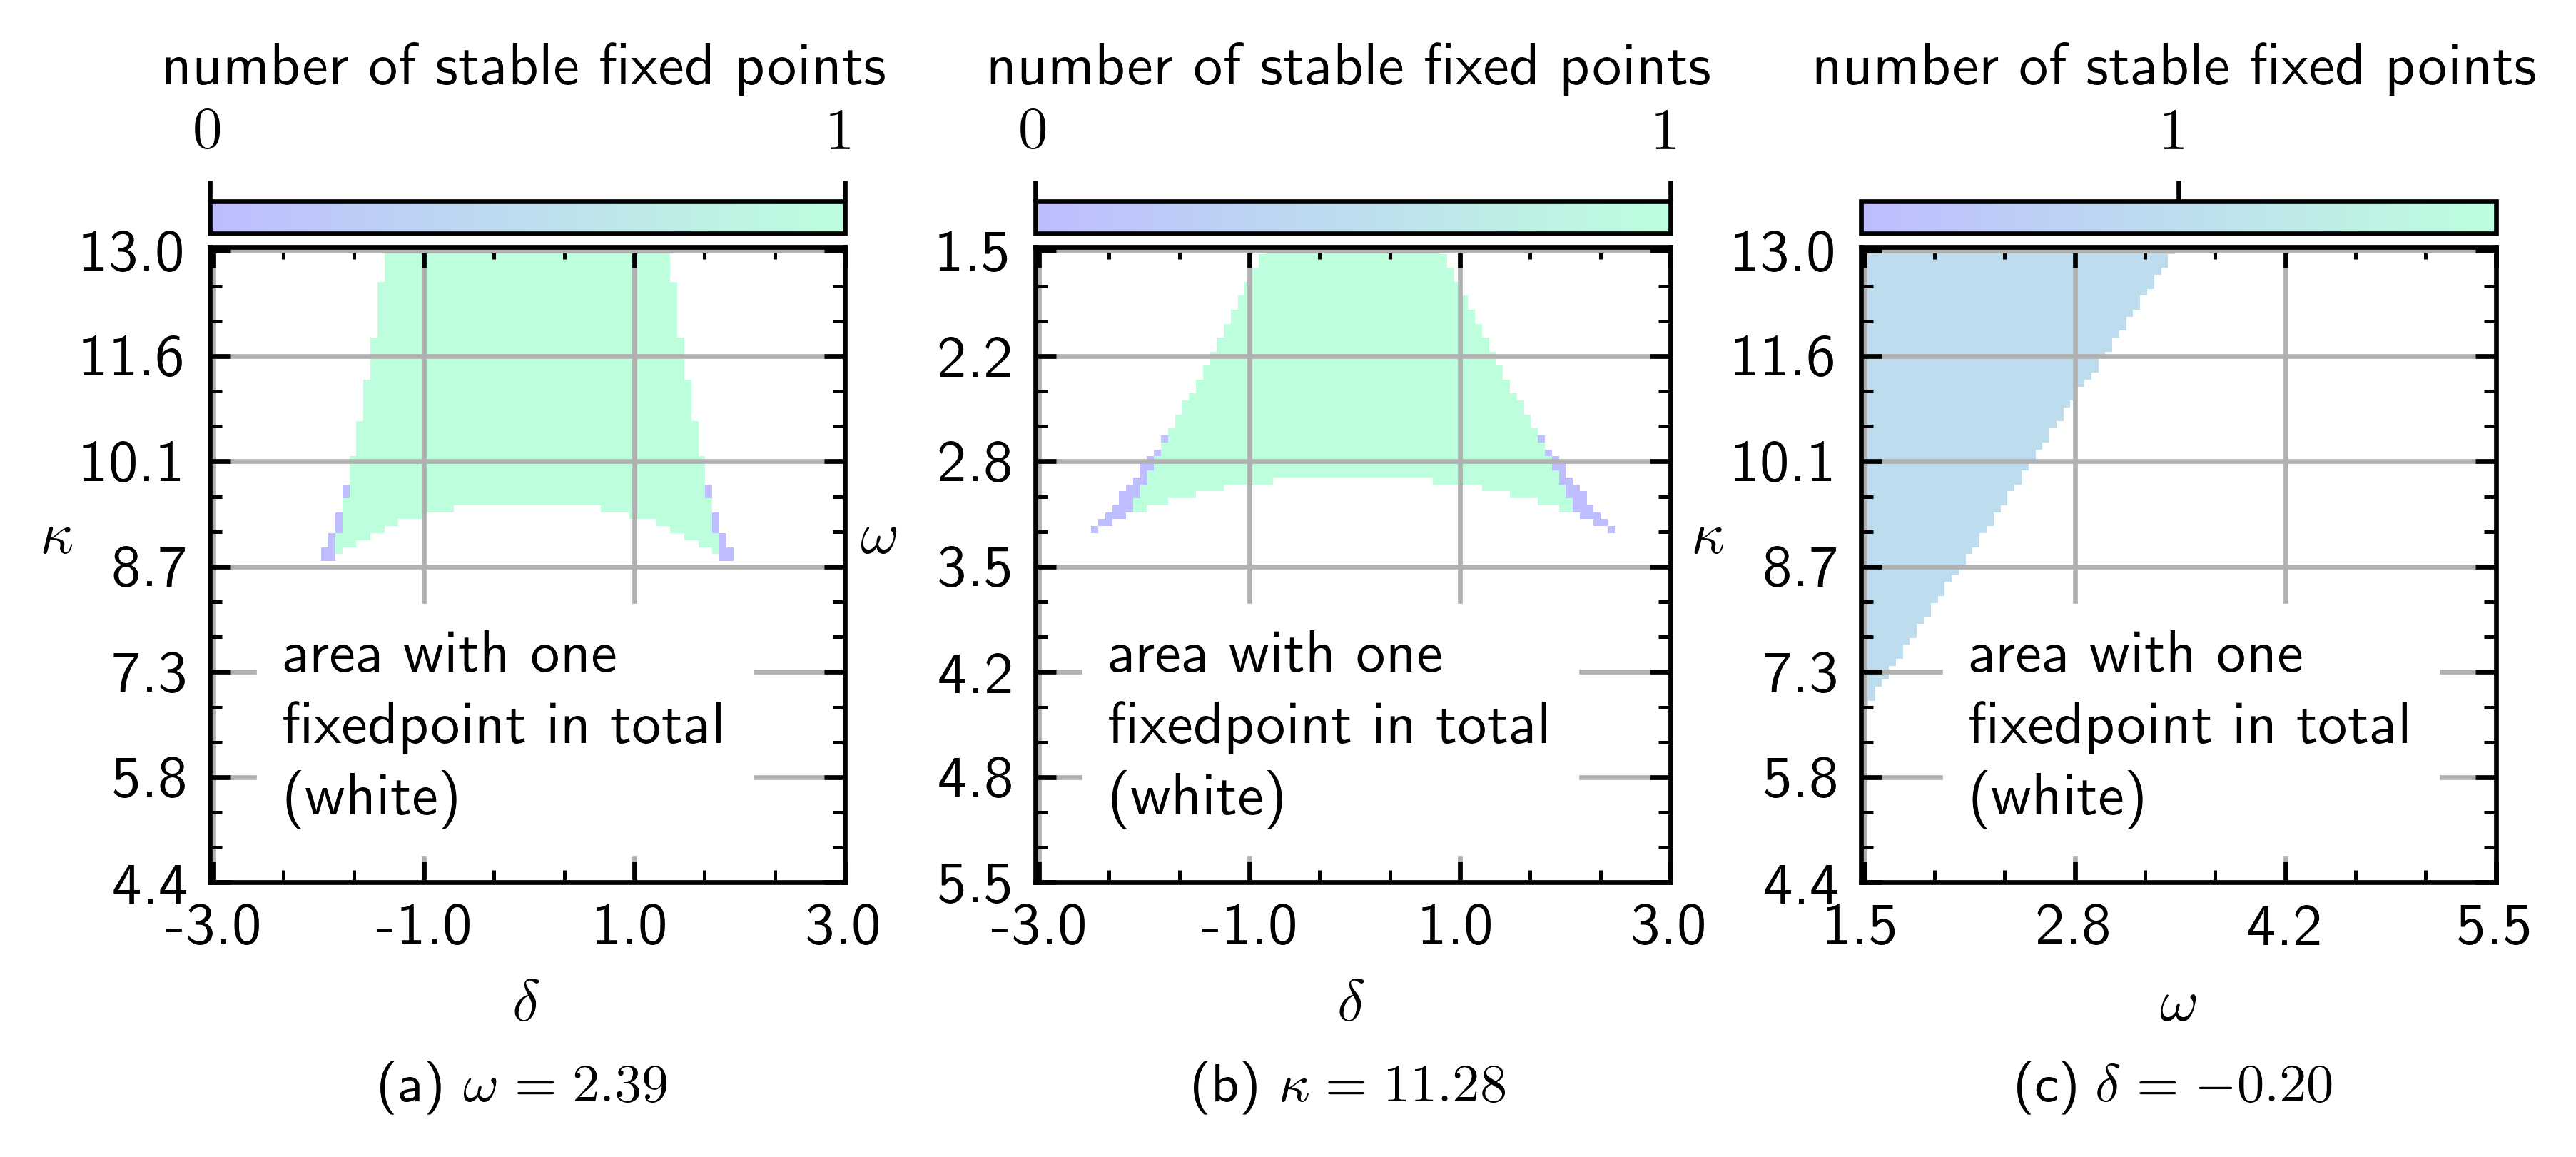
\includegraphics{pictures/numb_of_fixp_stabcuts2.png}
    \caption{Stability of the three stationary points. In this diagrams the area, in which three fixed points exist, is evaluated in more detail. So marked white are the the region, where only one fixed point is present, without distinction between stable and unstable ones. The purple sections indicate parameter constellations, for which there are 3 fixed points, but all of them are unstable, whereas green ((a)-(b)) and blue (c) indicate at least one stable fixed point. The diagrams are cuts through parameter space.}
    \label{fig:stability_cuts}
\end{figure}
In \figref{fig:stability_of_solutions} a region can be noticed, where 3 fixed points exist, but all of them are unstable. This is a consequence of the fact that for increasing $\kappa$ the number of stable fixed points decreases but at the same time the total number of stationary solutions grows. \figref{fig:stability_cuts} shows that those regions are located on the surface of the area with 3 stationary points, indicating a straight forward succession of phases, as parameters are altered.\\\\
Because the treatment of different coherent dephasing strengths does not deliver additional insights I will only consider a fixed dephasing at $\gamma=0.2$. A short treatment for varying $\gamma$ can be found in \appref{appendix:stability_gamma}.
% \begin{figure}[H]
%     \floatbox[{\capbeside%\captionsetup[capbesidefigure]%{labelsep=newline}%
%     \thisfloatsetup{capbesideposition={right,center},capbesidewidth=none}}]{figure}[\FBwidth]
%     {\caption{A 3D depiction of the area of 3 existing fixed points and their stability.\\\\
%     Marked with a color are the parameter configurations, where three stationary points exist. The Turquoise region at the edges mark non-stability. This shows that those parameter points lie on the surface of the region with three stationary points, and do not reach into the bulk of at least one stable fixed point, that is marked with a blueish purple. \\\\The assumption that in the absence of a stable stationary solution limit cycle can occur is in fact true. Through integration of the equations of motion one finds in those regions limit cycle and even quasi-periodic behavior. Some exemplary trajectories are found in the appendix.}}
%     {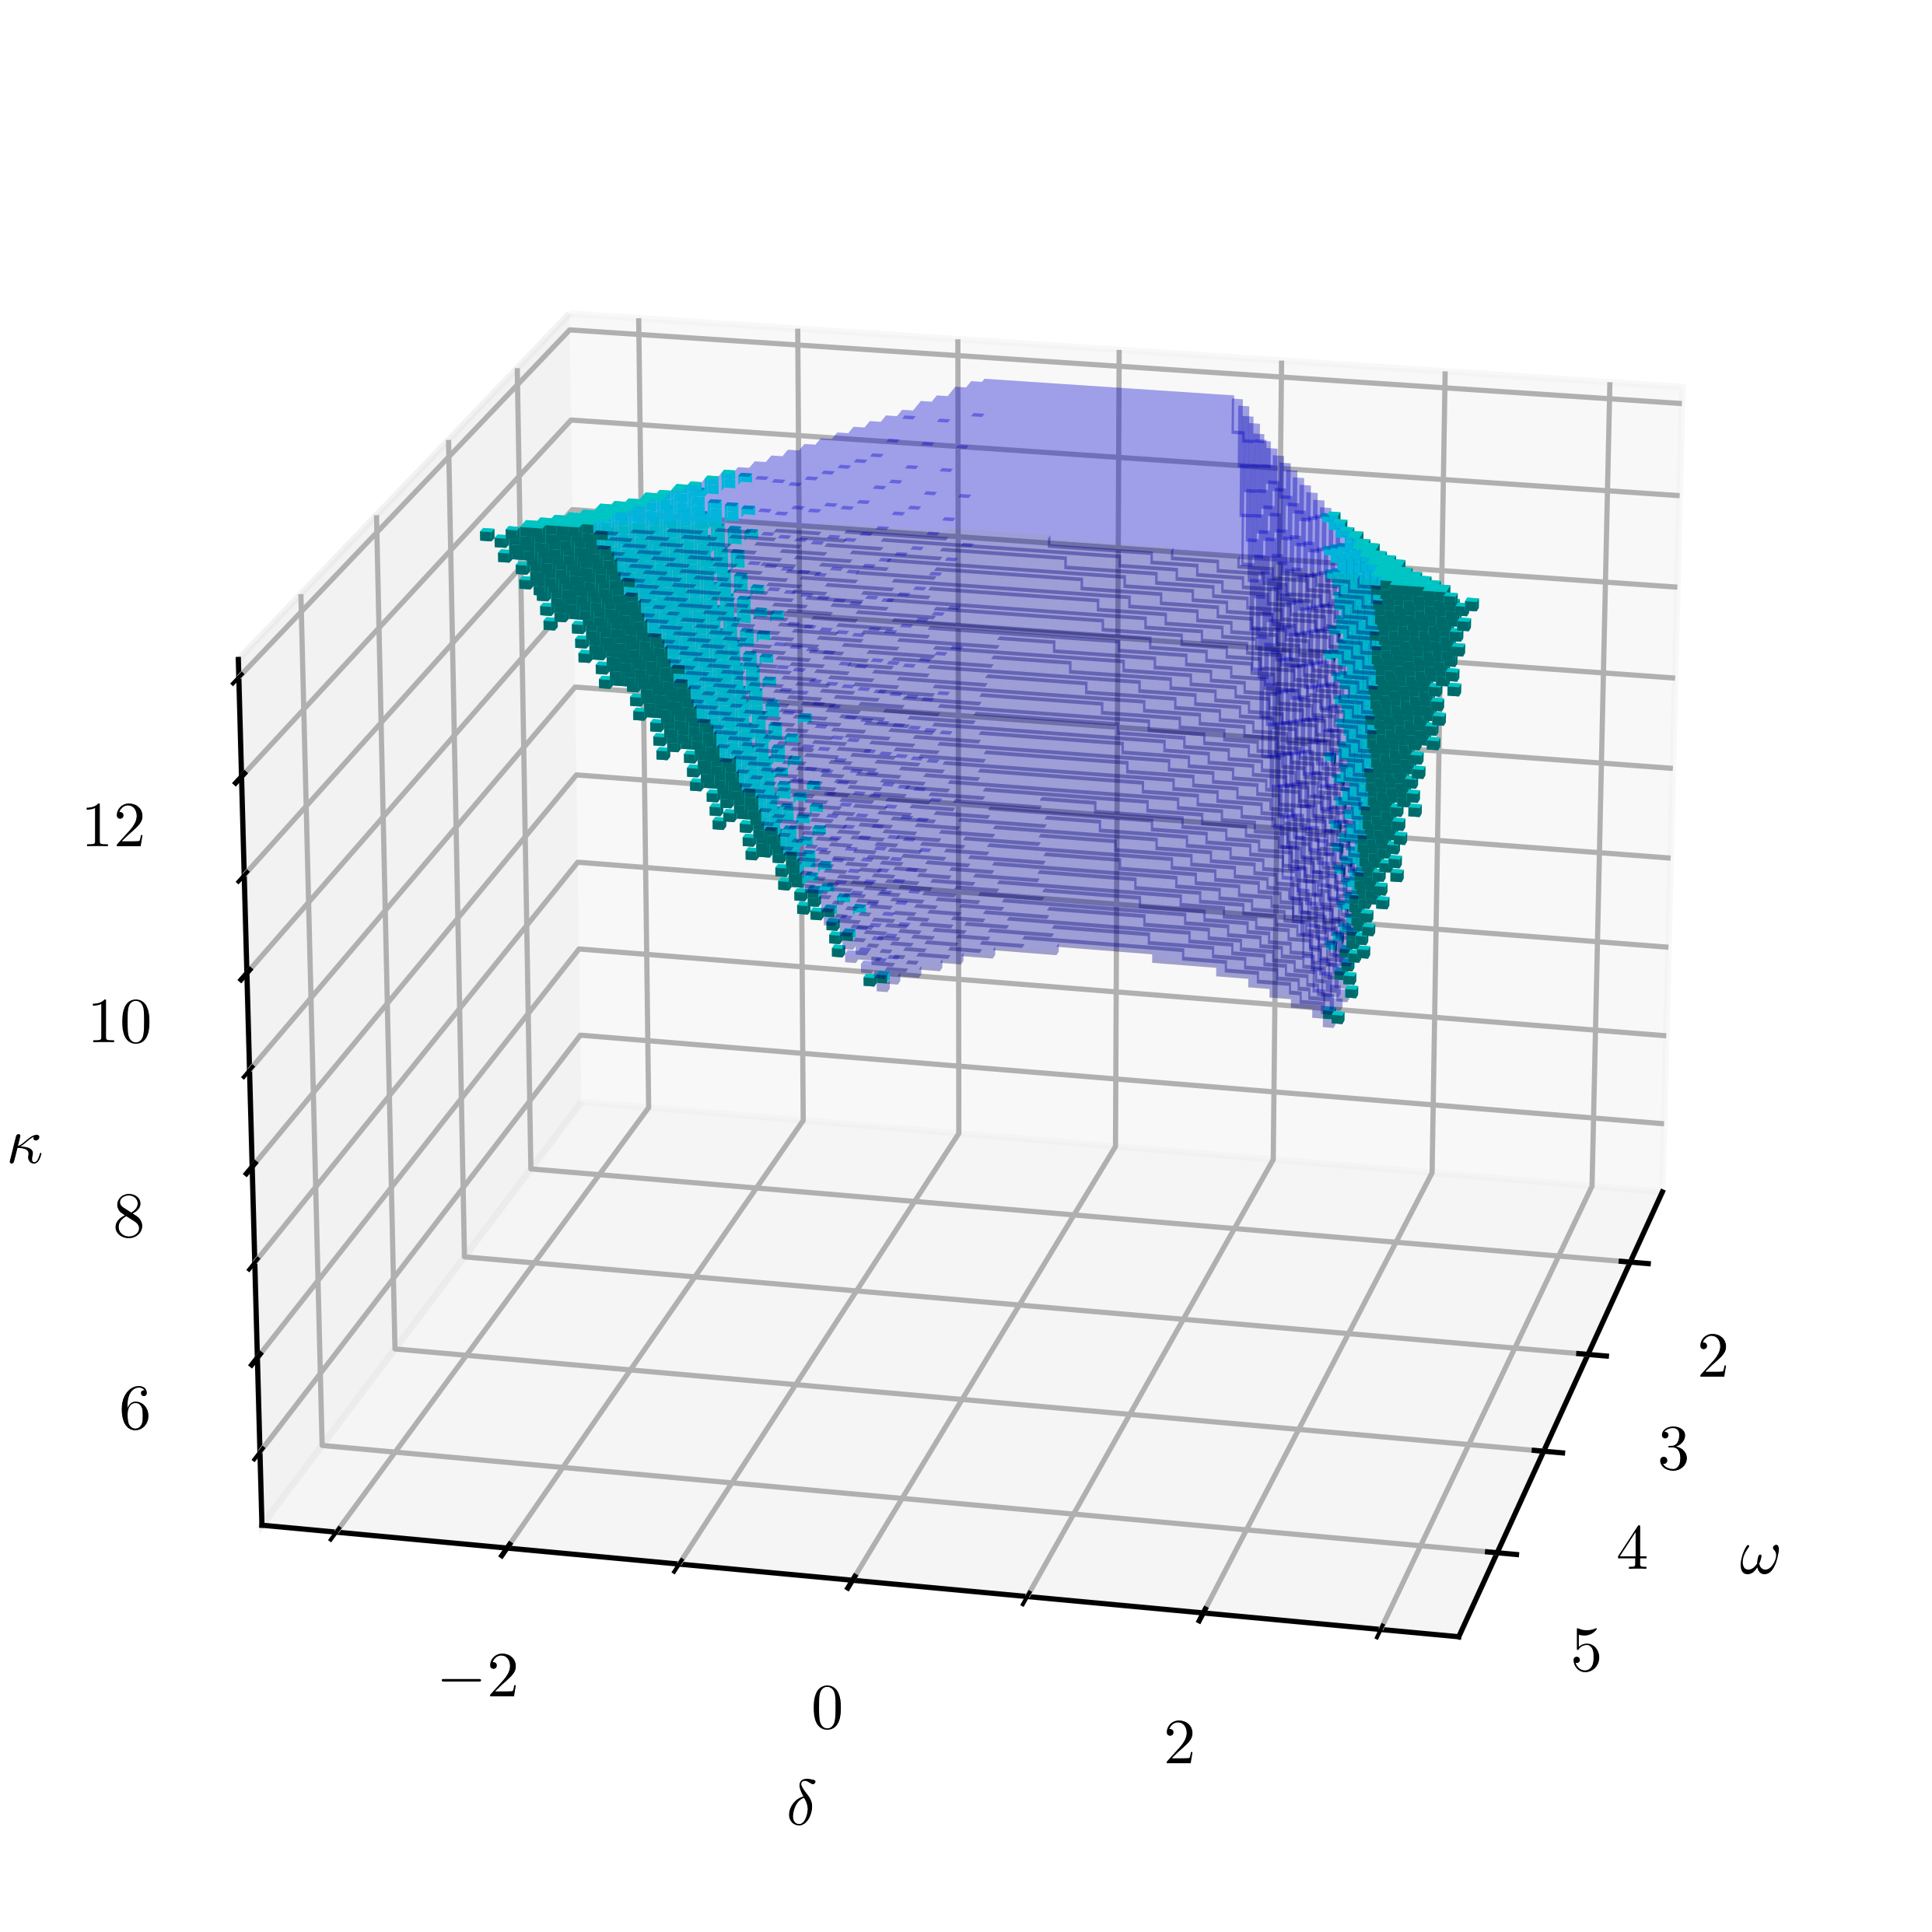
\includegraphics[scale=0.8]{pictures/numb_of_fixp_stab3d.png}}
%     \label{fig:fixp_stab3d}
%     %{\label{fig:num_of_fixp_criterium_BF}}
% \end{figure}
% \\\\
\subsection{Long-time behavior}
For long observation times the system will most likely be found in an attracting state, as already explained in \secref{sec:longterm_zerodel}. This can be a stationary solution or among others a time crystal state, meaning an undamped oscillation. Such states are in fact observable in our mean-field approach. 
\begin{figure}[H]
    % \vspace*{-1cm}
    \hspace*{-1.2cm}
    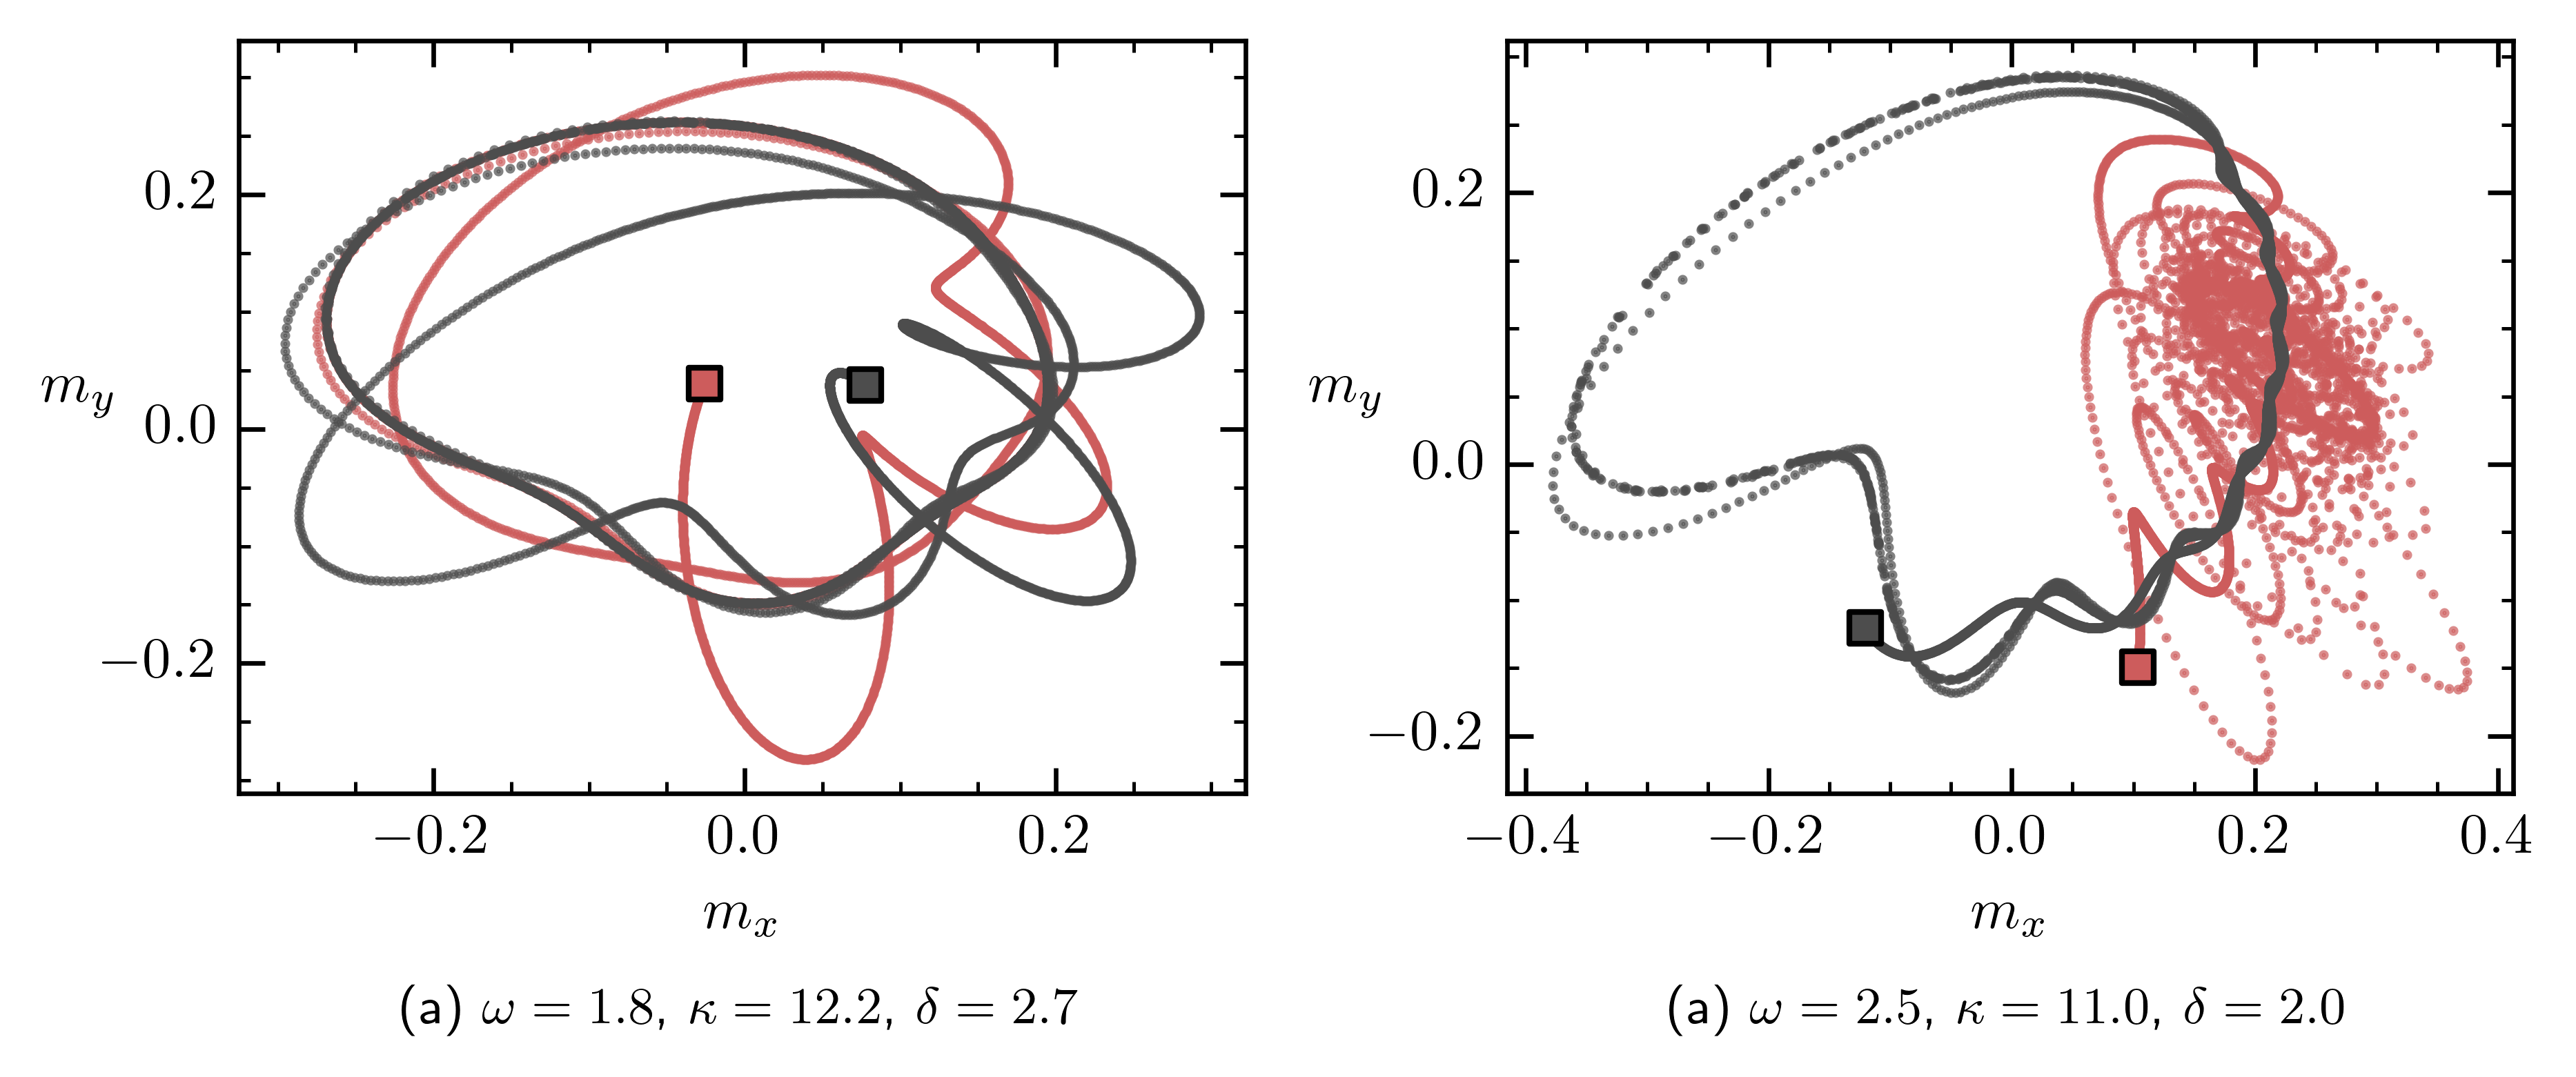
\includegraphics[scale=1]{pictures/lc_example.png}
    \caption{Two exemplary trajectories for two different parameter configurations. The starting points were picked randomly. The small squares with the black frame indicate the starting points of the system.}
    \label{fig:expl_lc}
\end{figure}
In \figref{fig:expl_lc} I plotted two exemplary trajectories, starting at random starting points, for two different parameter configurations. In \figref{fig:expl_lc} (a) one can see that after a convergence time both trajectories overlap each other. So there is only one limit cycle that the system is drawn to for both starting positions. Of course the phase of the oscillation depends on the start and can be different. But the trace of the trajectories in spin space coincides for long times. \\\\For the parameter configuration in \figref{fig:expl_lc} (b) at least two distinct patterns are possible for long times. The gray trajectory converges relatively fast to its limit cycle and hence looks cleaner. The rather messy appearance of the red trajectory stems from the long time it takes to approach its steady state. But both trajectories converge, as I have checked. In fact the darkest and broadest shaped ellipse that can be seen in red marks the limit cycle, the trajectory converges to.\\\\
The fact that two different limit cycles are possible long time states tells us that the system exhibits multistability for certain parameter constellation, in form of the presence of more than one attracting state. Where the system eventually ends up, is determined by the state at the beginning of the dynamics. In \appref{appendix:expl_traj} a few more exemplary long term states of the system are depicted for different parameter configurations.\newpage
The remaining part of this section is devoted to a further analysis of the evolution of multistability in parameter space and how the possible long-time states change with changing coupling constants. I will also be able to map some of the properties onto the language of synchronization.\\
A simple way to track the change of limit cycles as well as the rise of multistability is to observe the mean value of a limit cycle over its period.
\figref{fig:fixedpoint_colormap} has been created by plotting the stable stationary solution, where it exists, and in the other case the average over a period of a limit cycle.




% When examining the long term behavior of a system, a general point of interest is how the eventually occupied states shift and deform, when the parameters are changed. A simple observable in the context of time crystals is the mean value over a period of the limit cycle. 
\begin{figure}[H]
    % \vspace*{-1cm}
    \hspace*{-1.2cm}
    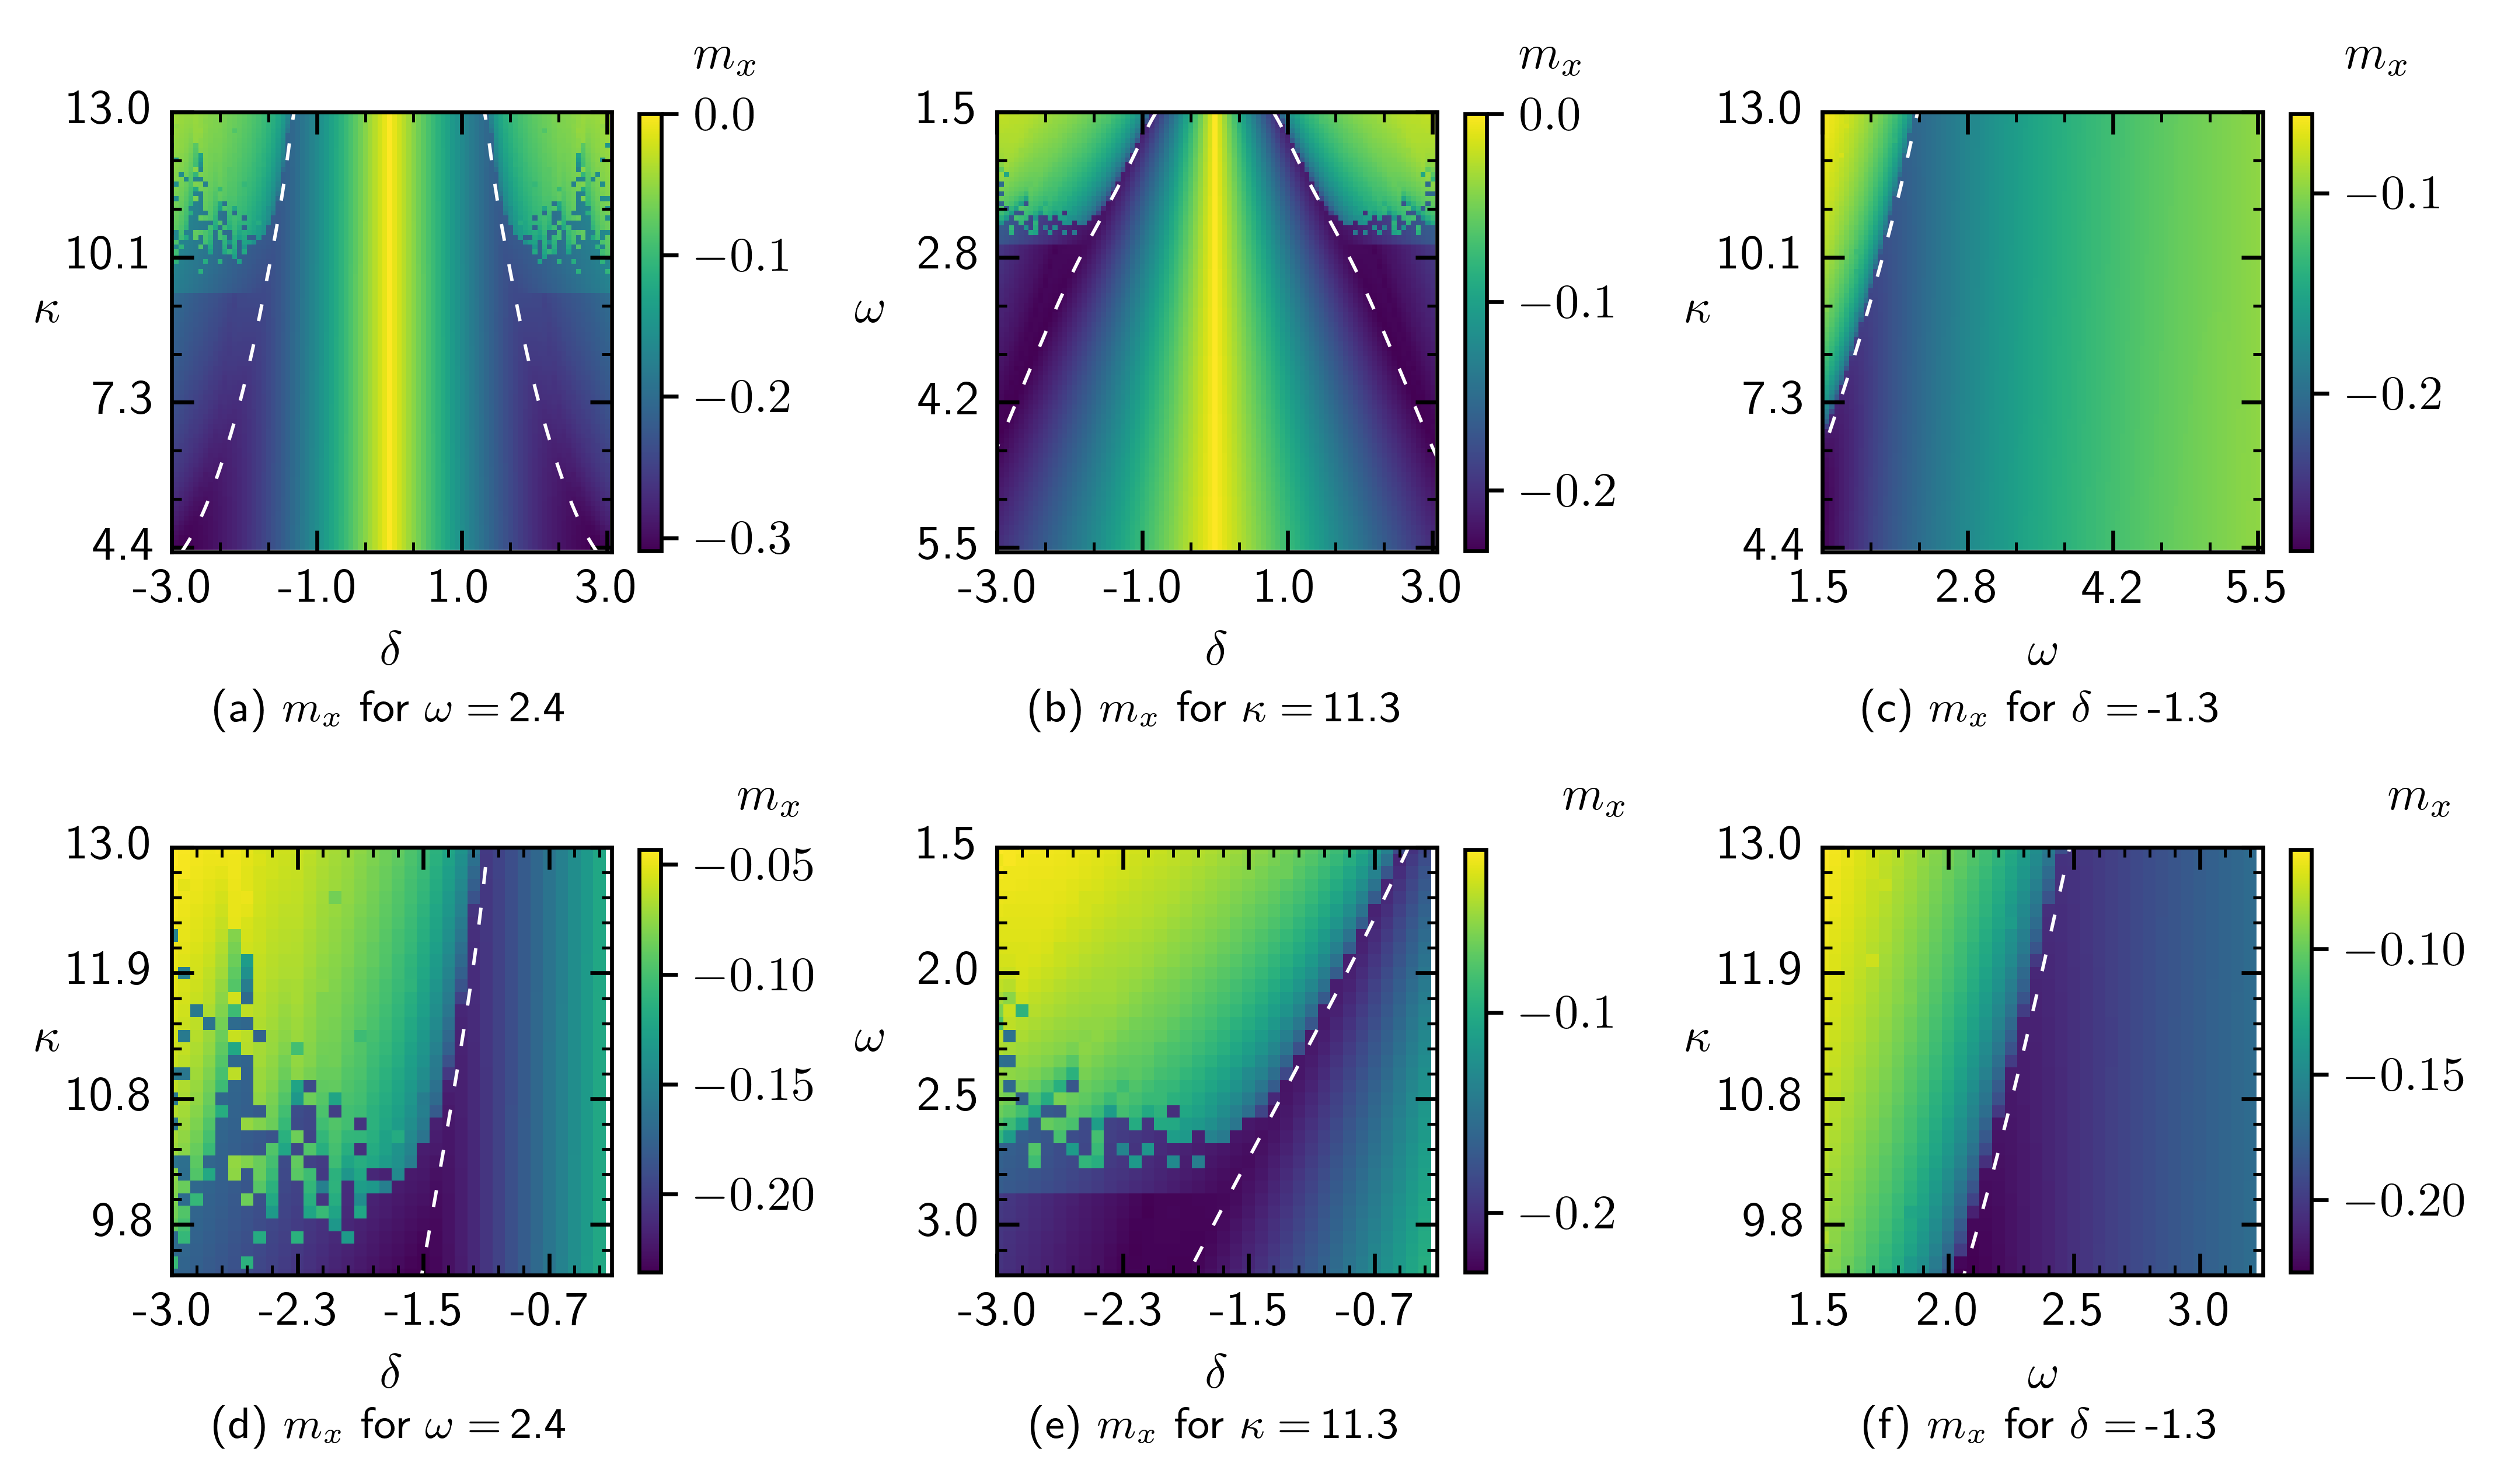
\includegraphics[scale=1]{pictures/stable_fixp_extended_withline_dashed.png}
    \caption{Shown is the $m_x$ component of the stable stationary points and of averaged limit cycles for different cuts through parameter space. Under each cut in the top row is a close-up of the interesting areas in the top left corners. the white dashed line separates the regions with one and from those with no stable fixed point. In the cases, where more than one limit cycle exists, I chose the one, whose average had the smallest $m_x$-value.}
    \label{fig:fixedpoint_colormap}
\end{figure}
By examining \figref{fig:fixedpoint_colormap} one can tell that transition from stationary steady states to the time crystal phase, which is marked by the white dashed line, is at some parameter points more smoothly than at others. The separation line has been computed by selecting the first point where there is no stable fixed point anymore, when passing through each line of the evaluated parameter grid in decreasing order of $\delta$, and fitting a polynomial of 4th degree to those points. Notice that as a result of this method the separation line lies inside the time crystal phase. Also because of the approximate nature of this determination, the line should only serve as a orientation, where the phase separation is located.\\\\
For the cuts with constant $\kappa$ and constant $\omega$, the area, where limit cycles exist, can be roughly divided into two regions. For one region, as already mentioned the transition from the stationary phase is very smooth, whereas for the other region, there is significant change in the average value of the long-time states to the nearby parameter configurations where stationary solutions exist. Multistability has also its influence on the appearance of the diagram. Where it occurs, I plotted in \figref{fig:fixedpoint_colormap} the averaged limit cycles with smallest $m_x$-value. \\What also stands out is that the phase plot in this part of the parameter space is very fragmented. The biggest effect of this impression is that for the generation of this diagram too few starting points have been chosen, to detect all present limit cycles. Another important factor was, that in order to integrate up to long times without having too much error, one has to choose the precision of the integrator very high, which has not been done, when originally generating \figref{fig:fixedpoint_colormap}. \\Because of the high numerical expense it takes to determine enough trajectories of the system up to a sufficiently large time with good precision, I have decided to redo the diagram in more detail only for a selected area in the plane of $\omega=2.3889$. An additional remark has to be made regarding \figref{fig:fixedpoint_colormap}. In some of the plots a sudden but slight jump in the color temperature is noticeable. This stems from the fact that already in those plots a minor adjustment of precision has been made for the critical regions. %The white dashed separation line between limit cycles and stationary points has been determined by collecting the border points where just no stable stationary point exists anymore and fitting a spline to it. Because of the low resolution of considered parameter constellations the curve should serve more as an approximate locater of the border between limit cycles and fixed points than a definite cut.
\subsubsection{Synchronization}\label{sec:synchronization}
Despite all of the mentioned constraints, the diagram is valid for most of the shown area, as only the change from the one limit cycle phase to the multistability region has some artefact. Thus I will focus now on the information that can be retrieved from the valid parts of the diagram.\\%, due to the above mentioned reasons. 
The shape of the white dashed separation line in the $\omega$-$\delta$-diagram reminds of the typical division of states for contexts, in which synchronization effects are observable. Synchronization is the adaption of two oscillating systems to each other, which are coupled through a weak interaction. In our case the two synchronizing parts are the system on the one hand and the driving laser on the other. As the driving laser is not affected by the system, only the latter can adapt. Hence synchronization takes place, when the system oscillates with the same frequency as the laser. This phenomenon is called frequency locking, because the frequency of the system is locked to the one of the laser. As the equations of motion are formulated in the rotating frame of the laser, see \secref{sec:theory}, the dynamics in case of frequency locking take the form of stationary points. In order to being able to speak of synchronization, a few conditions have to be met\cite{synchronization}.
\begin{itemize}
    \item The coupling between the two systems has to be weak enough to speak of non-trivial influence.
    \item Both systems have to be able to maintain autonomous oscillations, if decoupled.
    \item If the original frequency of one of the systems is altered, this has to have an effect on the resulting common frequency, that arises due to the coupling.
\end{itemize}
As the both regions of limit cycles as well as stationary points extent to small values of $\omega$, i.e. small interaction between laser and system, in those areas the condition of weak coupling is satisfied. Also the last condition of changing locked frequency with change of the systems is fulfilled. I have already said, that the laser in our formalism is not influenced by the system. Therefore only the system can follow the change in laser frequency. As the system exhibits stationary states in a certain interval around $\delta=0$, what has been confirmed in \secref{sec:stab_3D}, the system is locked to the oscillation of the laser for changing laser frequencies. In order to confirm autonomous oscillations of the system without laser driving, one has to remove the driving from the formalism, which is not trivial. The Hamiltonian for this case reads
\begin{align*}
    H &= \frac{\omega_0}{2}\,J_z +\alpha\,(J_+a + J_-a^\dagger)+ \beta\,J_z\,(b^\dagger+b)+\xi\,\sum_{i=1}^N\,(\sigma_i^-c_i^\dagger+\sigma_i^+c_i)
\end{align*}
As a consequence of not having to perform a transformation into the rotating frame of the laser, the bosonic ancilla operators, are defined slightly differently, i.e. related to a factor $\propto\exp(i\omega_0t)$. But this really does not change the quality of the dynamics. It becomes obvious that the same dynamics can be achieved by setting in the original Hamiltonian with driving $\omega=0$ and $\delta=\omega_0$. Examining trajectories for these parameter configurations one can find limit cycles arise. Thus the system is able to maintain oscillations even without external laser driving, hence satisfying the remaining condition for synchronization. As mentioned earlier the transition line between fixed points and time crystal phase, has a typical property of the phase locking effect. The more the frequencies of the involved systems differs, the stronger the coupling between them has to be to achieve synchronization. 
\subsubsection{Multistability}\label{sec:multistability}
Having thus found an enriching correspondence of the found phase plot to synchronization effects, I want to turn to the discussion of multistability, that occurs in the time crystal phase. For this analysis I have redone the diagram that shows the change of the average value of a limit cycle over a period for the plane with $\omega=2.3889$. It is shown in \figref{fig:precise_multistab2d}.
\begin{figure}[H]
    % \vspace*{-1cm}
    \hspace*{-1.2cm}
    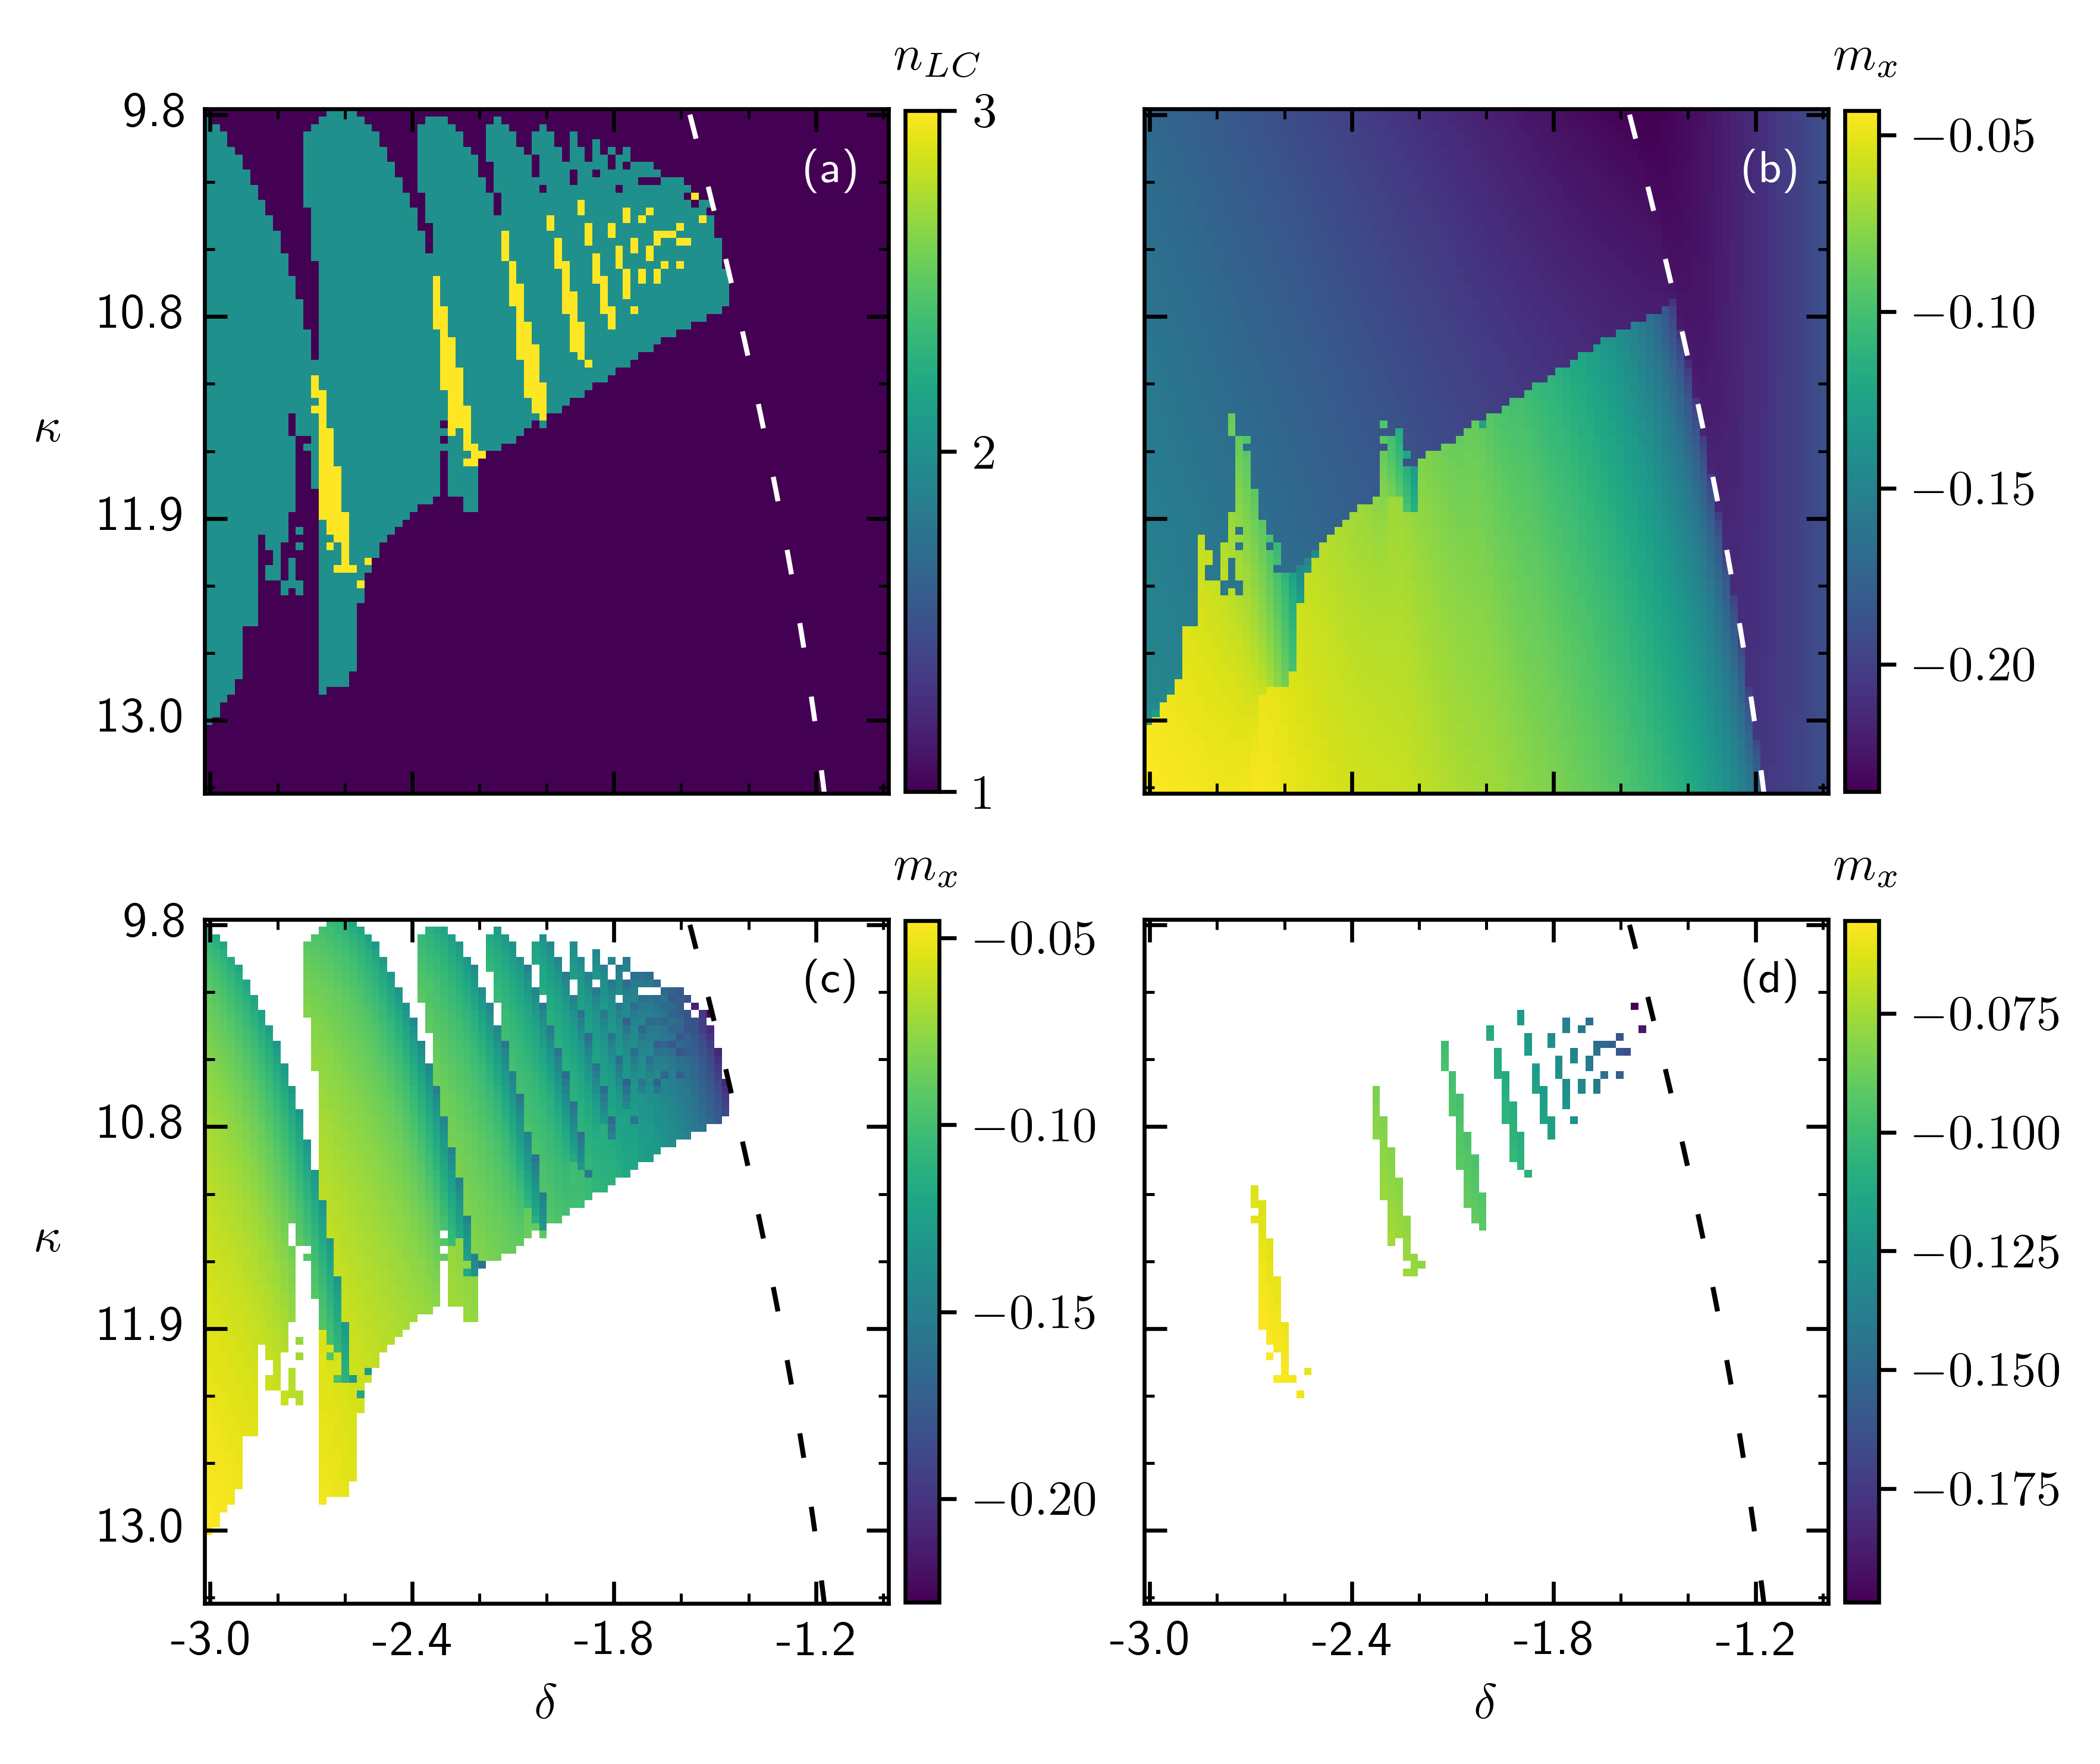
\includegraphics{pictures/limit_cycle_mean.png}
    \caption{multistability phases. In (a) $n_{LC}$ measures the number of different limit cycles. The dashed line, which also present in the other three plots, separates the region of fixed points (right) from that where stable long-time oscillations exist (to the left of the line). The values of the fixed point as well the averages of the $m_x$-component of the spin over a period are shown in diagrams (b)-(d). The plotted averages have been chosen in increasing order of their value, i.e in (b) the smallest values of $m_x$ have been plotted and in (d) the largest.}
    \label{fig:precise_multistab2d}
\end{figure}
\figref{fig:precise_multistab2d}(a) shows the number of different limit cycles. It was determined by computing the average value over the period of a cycle of the total spin. The criteria by which stable oscillations have been differentiated from each other was a distance of mean total spin of at least $0.005$. It is found that up to three different limit cycles are approached for the same parameter configuration depending on the starting points of the system. Intriguingly a repeating pattern shows when the detuning is changed. Period and amplitude of this oscillation-like behavior is decreasing with shrinking $\delta$. \\\\What is also interesting is that the sharp transition in the mean value of the $m_x$-component of the spin is not due to the rise of multistability. Multistability rather accompanies the change in mean long-time spin. Passing through parameter space from small to big $\kappa$ one can say the following. Where more than one limit cycle exists, one of them keeps up the smooth course of average spin. When moving further in parameter space up to the area, where again only one stable oscillation exists, only those oscillations survive, which continue the previous course of average spin more abruptly (\figref{fig:precise_multistab2d}(b)). Hence the multistability appears at a transition in magnitude of the averaged $m_x$-value, where a region of elevated $m_x$-value stretches out a comb of additional long time states beyond a rather sharp border. I want to explicitly mention that, what the above figure suggests - namely that the comb of \figref{fig:precise_multistab2d}(c) expands the bright section of \figref{fig:precise_multistab2d}(b) - is in  fact true.\\\\
Expanding the analysis I want to look in more detail to the behavior of multistability as the detuning is changed. Therefore I picked two one-dimensional cuts through parameter space. They are marked in \figref{fig:delta_cut_traj}. One line is picked in the area where a repeating pattern in $\delta$ is observed. Another one has been selected in the area where the number of limit cycles exhibits a large incision and despite larger integration precision, the exact border could not be resolved well. \\\\
% \begin{figure}[H]
%     % \vspace*{-1cm}
%     \hspace*{-1.2cm}
%     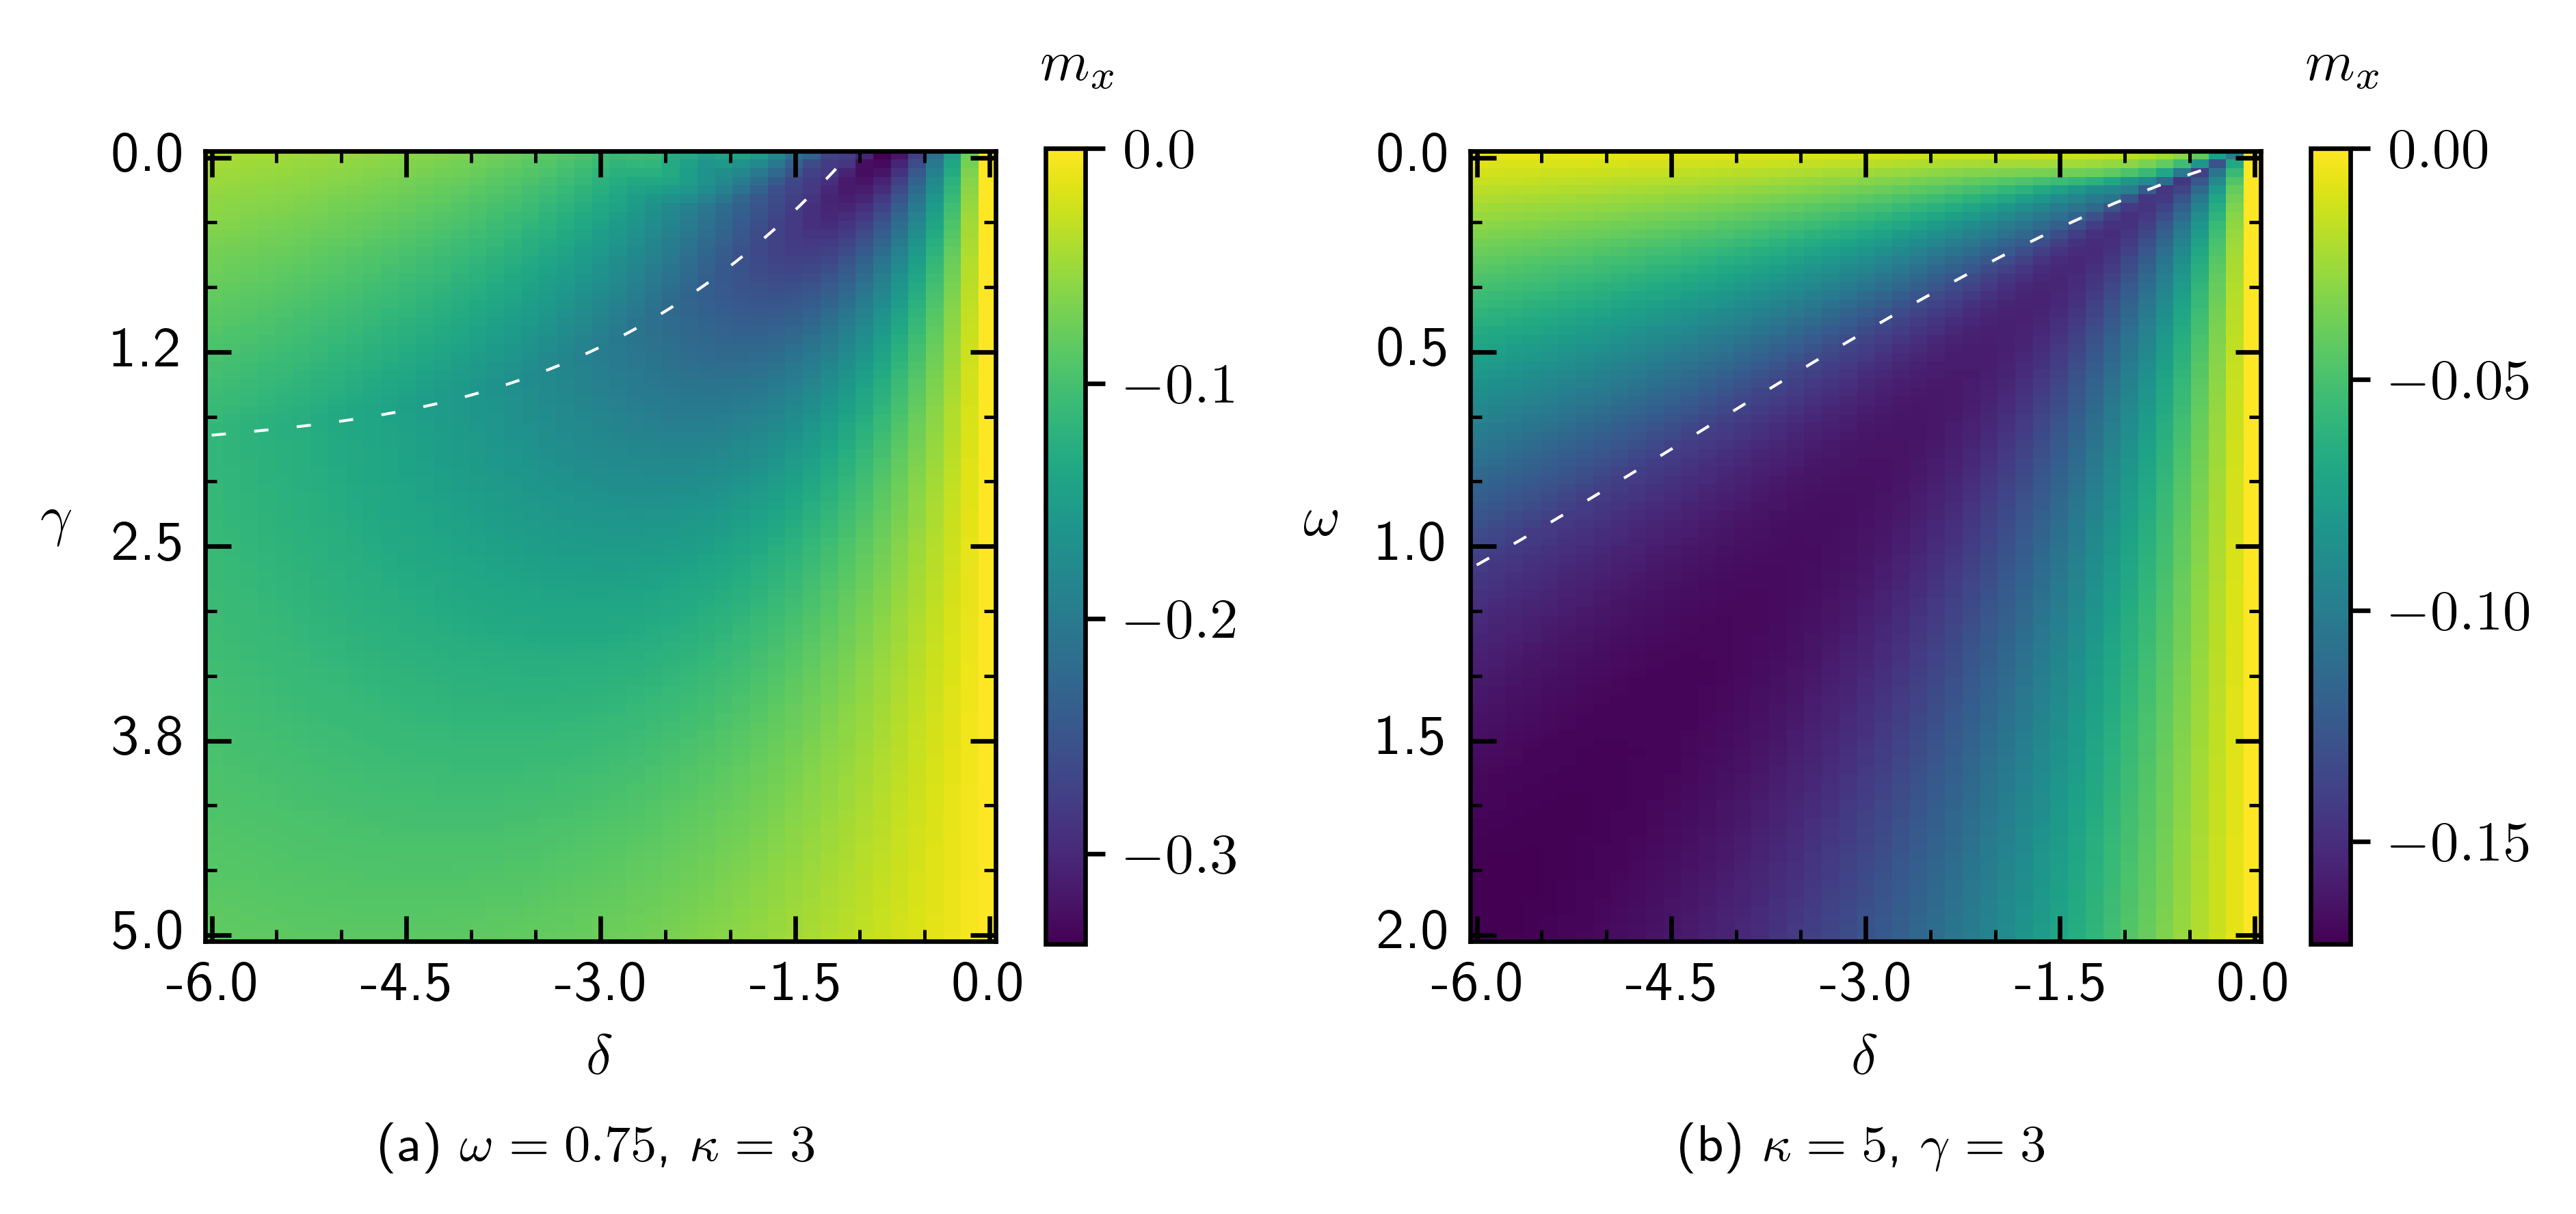
\includegraphics{pictures/limit_cycle_mean_gw.png}
%     \caption{$n_{LC}$ measures the number of different limit cycles.}
%     
% \end{figure}
\begin{figure}[H]
    % \vspace*{-1cm}
    % \hspace*{-1.2cm}
    \caption{cut locations. Drawn in white are the paths in parameter space, where the the course of multistability is examined in greater detail and resolution. The upper line has its position at $\kappa=10.12$ and the lower line is located at $\kappa=11.9$. $\omega$ has its value at $2.3889$. The white dashed line again marks the onset of stable stationary solutions for smaller detuning values.}
    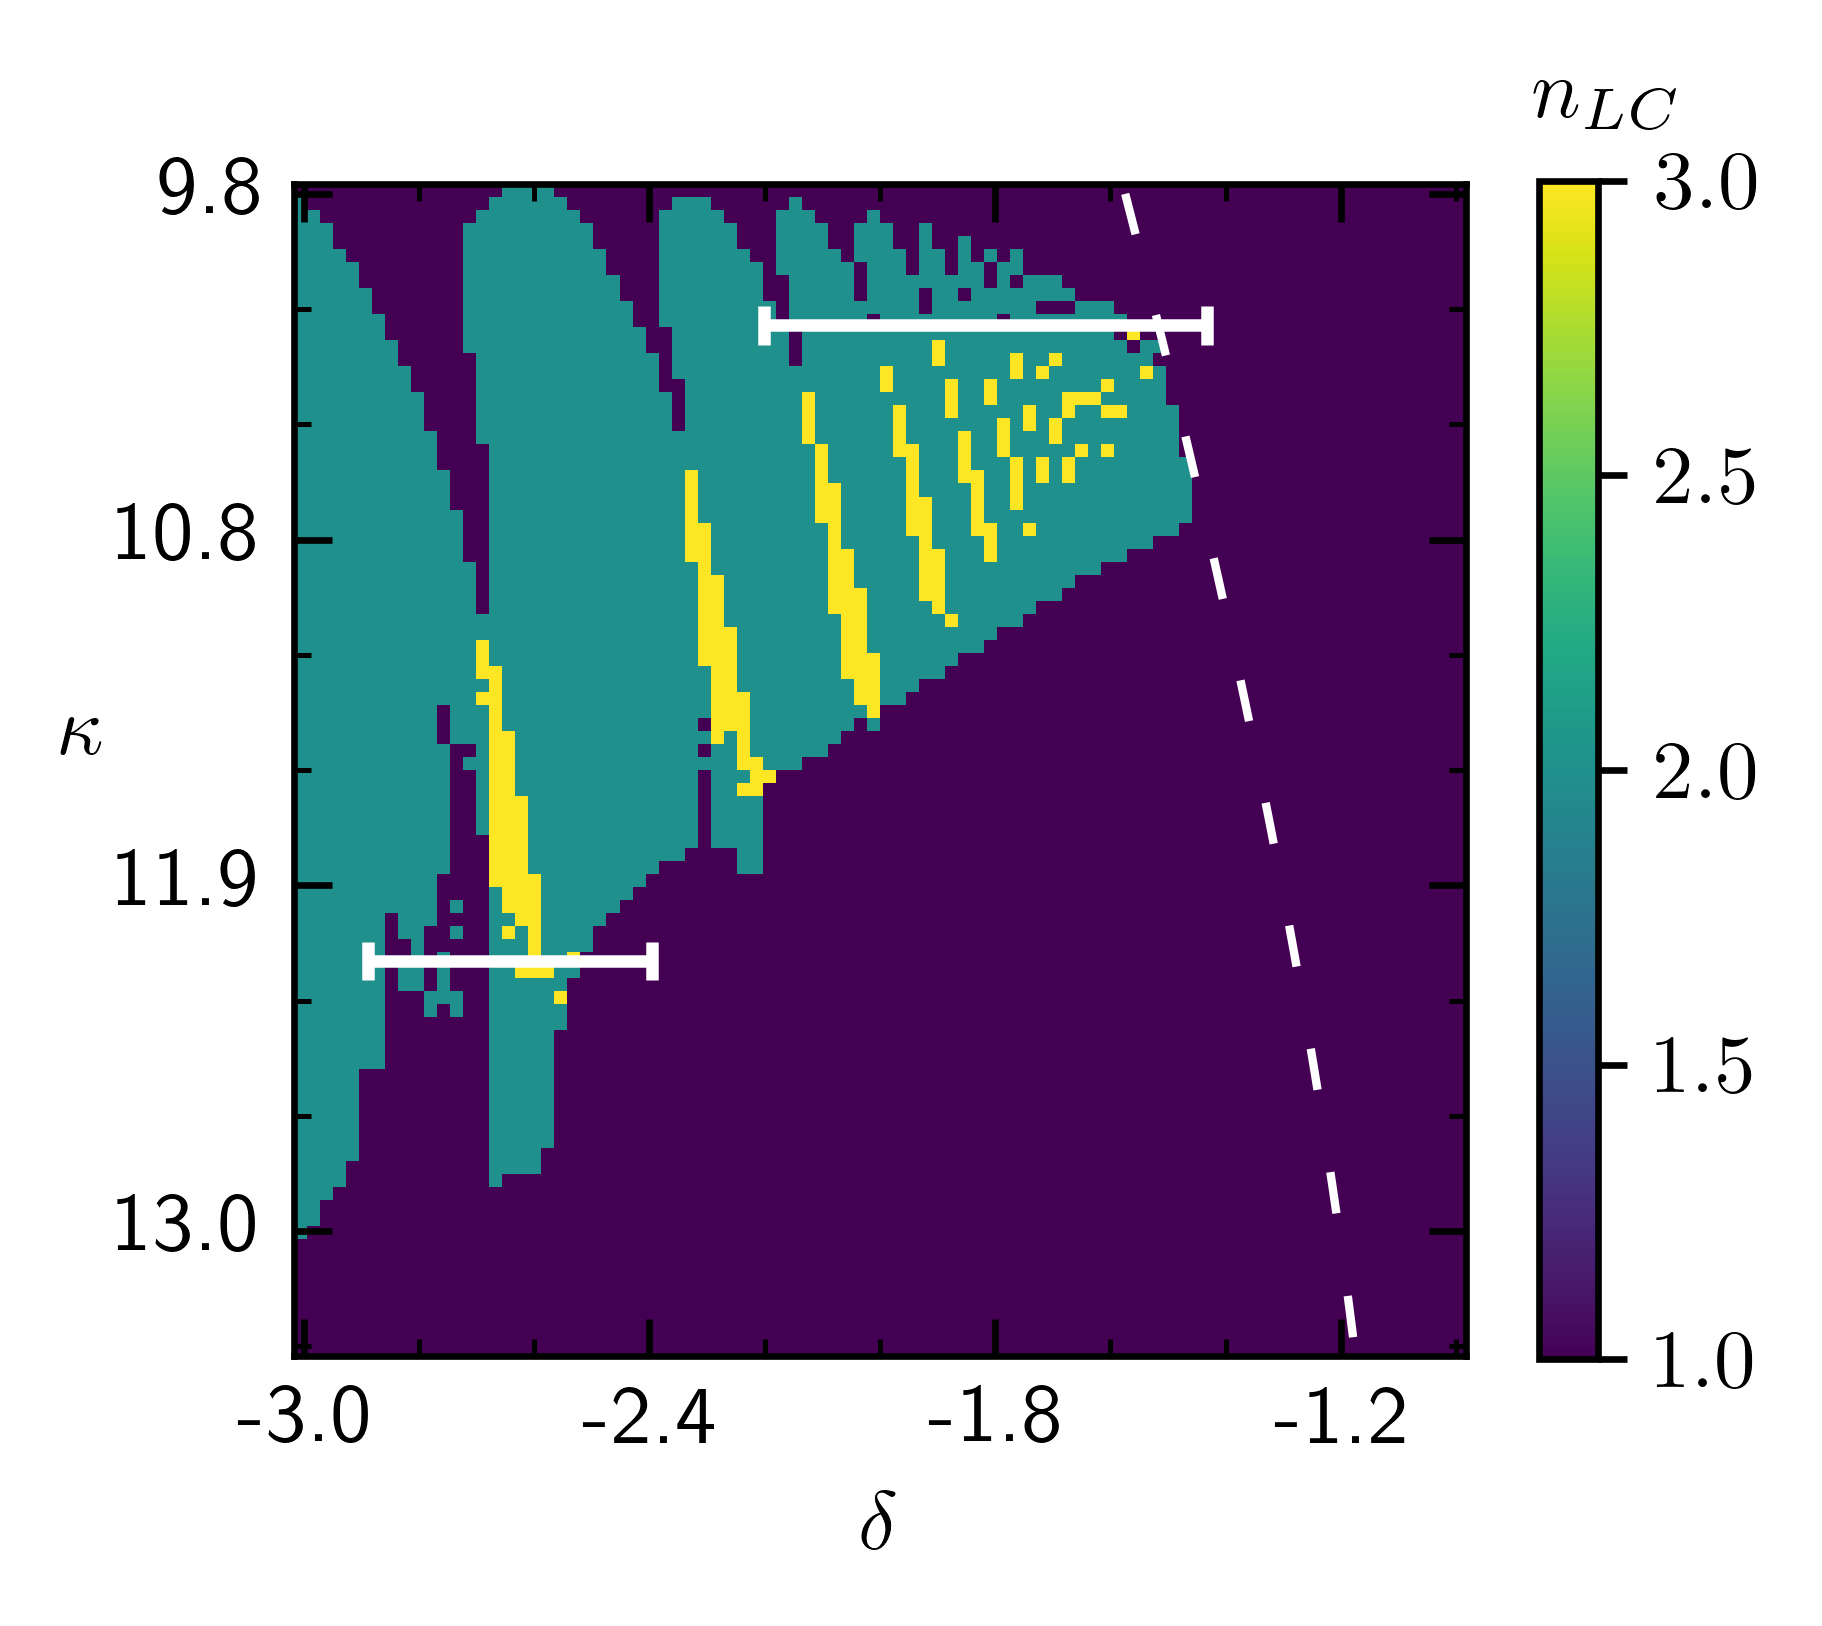
\includegraphics{pictures/multistab_cuts.png}
    \label{fig:delta_cut_traj}
\end{figure}


\begin{figure}[H]
    % \vspace*{-1cm}
    \hspace*{-1.2cm}
    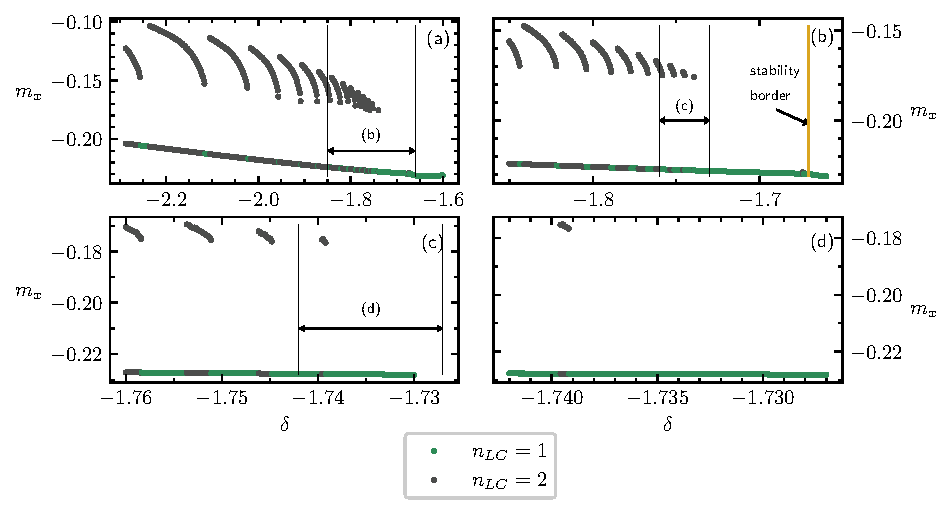
\includegraphics{pictures/multistab_line.pdf}
    \caption{One dimensional multistability cuts for the oscillatory area. Drawn are the $m_x$-values of trajectories averaged over a period of the limit cycle. In (a) 400 different values for the detuning have been considered. Particularly interesting looking sub-intervals have been identified and shown in greater detail in figures (b)-(d). All of them show the average of all the possible long-time states for 750 different $\delta$-values. Throughout the figure $\kappa=10.12$ and $\omega=2.39$.}
    \label{fig:osci_cut}
\end{figure}
The cut for the former region, where oscillatory-like patterns are found is depicted in \figref{fig:osci_cut}. It can be observed that a similar pattern repeats itself. Following the depiction of the averaged limit cycles with decreasing detuning, the distance in $\delta$ between each pattern shrinks, as well as the range of $m_x$, that each section of multistability covers. \\\figref{fig:osci_cut}(d) also shows that the pattern gets extinct at $\delta\approx-1.74$ and hence a good way before the onset of stability or synchronization. I have chosen a high resolution of $1000$ values for the detuning between $-1.742<\delta<-1.727$. I expect this number of grid points to be sufficient in order to detect an additional instance of the aforementioned pattern, if it existed. But further investigation is necessary to answer this question finally. Another observation that can be made is that the number of fixed points jumps discontinuously in the detuning.\\\\
I want to end the discussion of multistability with the close-up that is shown in \figref{fig:delcut_bay}. It depicts a cut through the area where a wedge of singular stability is  located between two regions, in which two and three different limit cycles exist. The cut through this wedge shows highly discontinuous behavior in $\delta$. One finds two uninterrupted branches at larger $m_x$-values. They coexist for certain values of detuning, but are not connected. The third branch with smallest $x$-component of the collective spin is very discontinuous. It contains unconnected parts of variable size, and goes over to a combination of three graphs of different character, which is depicted in \figref{fig:delcut_bay}(d). \\\\Understanding the behavior of \figref{fig:osci_cut} and \figref{fig:delcut_bay} is an outlook to future work, as it is out of the scope of this project.
\begin{figure}[H]
    % \vspace*{-1cm}
    \hspace*{-1.2cm}
    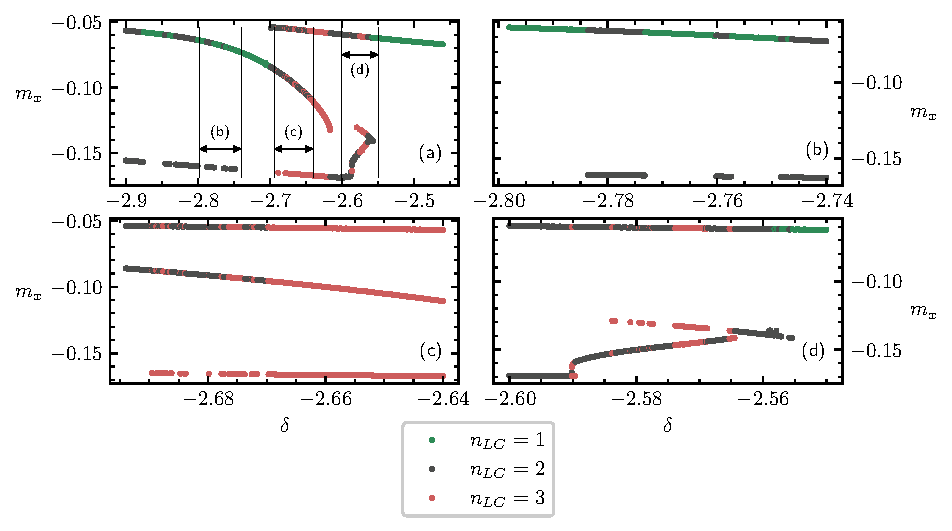
\includegraphics{pictures/multistab_line_bay.pdf}
    \caption{One dimensional cuts for the region where the multistability is incised (See \figref{fig:delta_cut_traj}). Drawn are the $m_x$-values of trajectories averaged over a period of the limit cycle. Subfigure (a) shows a wide cut through the incision. For that 1000 different values for the detuning have been considered. (b)-(d) are close up diagrams of regions marked in (a). All of them show the average of all the possible long-time states for 750 different $\delta$-values. Throughout the figure $\kappa=11.9$ and $\omega=2.39$.}
    \label{fig:delcut_bay}
\end{figure}
This section constituted the main part of the thesis. The full model with present detuning has been examined with respect to stability and long-time states. I have learned in \secref{sec:stab_3D} that the system exhibits regions, in which the collective spin always ends up at stable stationary points after a certain time of convergence. These stationary solutions can be explained by synchronization, where the system adapts its oscillations to the frequency of the laser, see \secref{sec:synchronization}. \\Outside the regions of synchronization the system performs oscillations, which break free from the complete adaption to the external driving. The hence resulting limit cycles have been analyzed regarding to their transformation as parameters are changed, \secref{sec:multistability}. It was found that multistability arises, accompanying a change of magnitude of the mean spin value. \\Further was observed that the number of different limit cycles, that exist for a certain parameter configuration, jumps discontinuously in parameter space. Especially rich behavior is found at such transitions. Repeating and highly discontinuous patterns could be observed, when the detuning was altered. I will now close the thesis with a total summary of its findings followed by a brief outlook to possible future investigations.


% \subsection{Basin of attraction}
% \begin{figure}[H]
%     % \vspace*{-1cm}
%     \hspace*{-1.2cm}
%     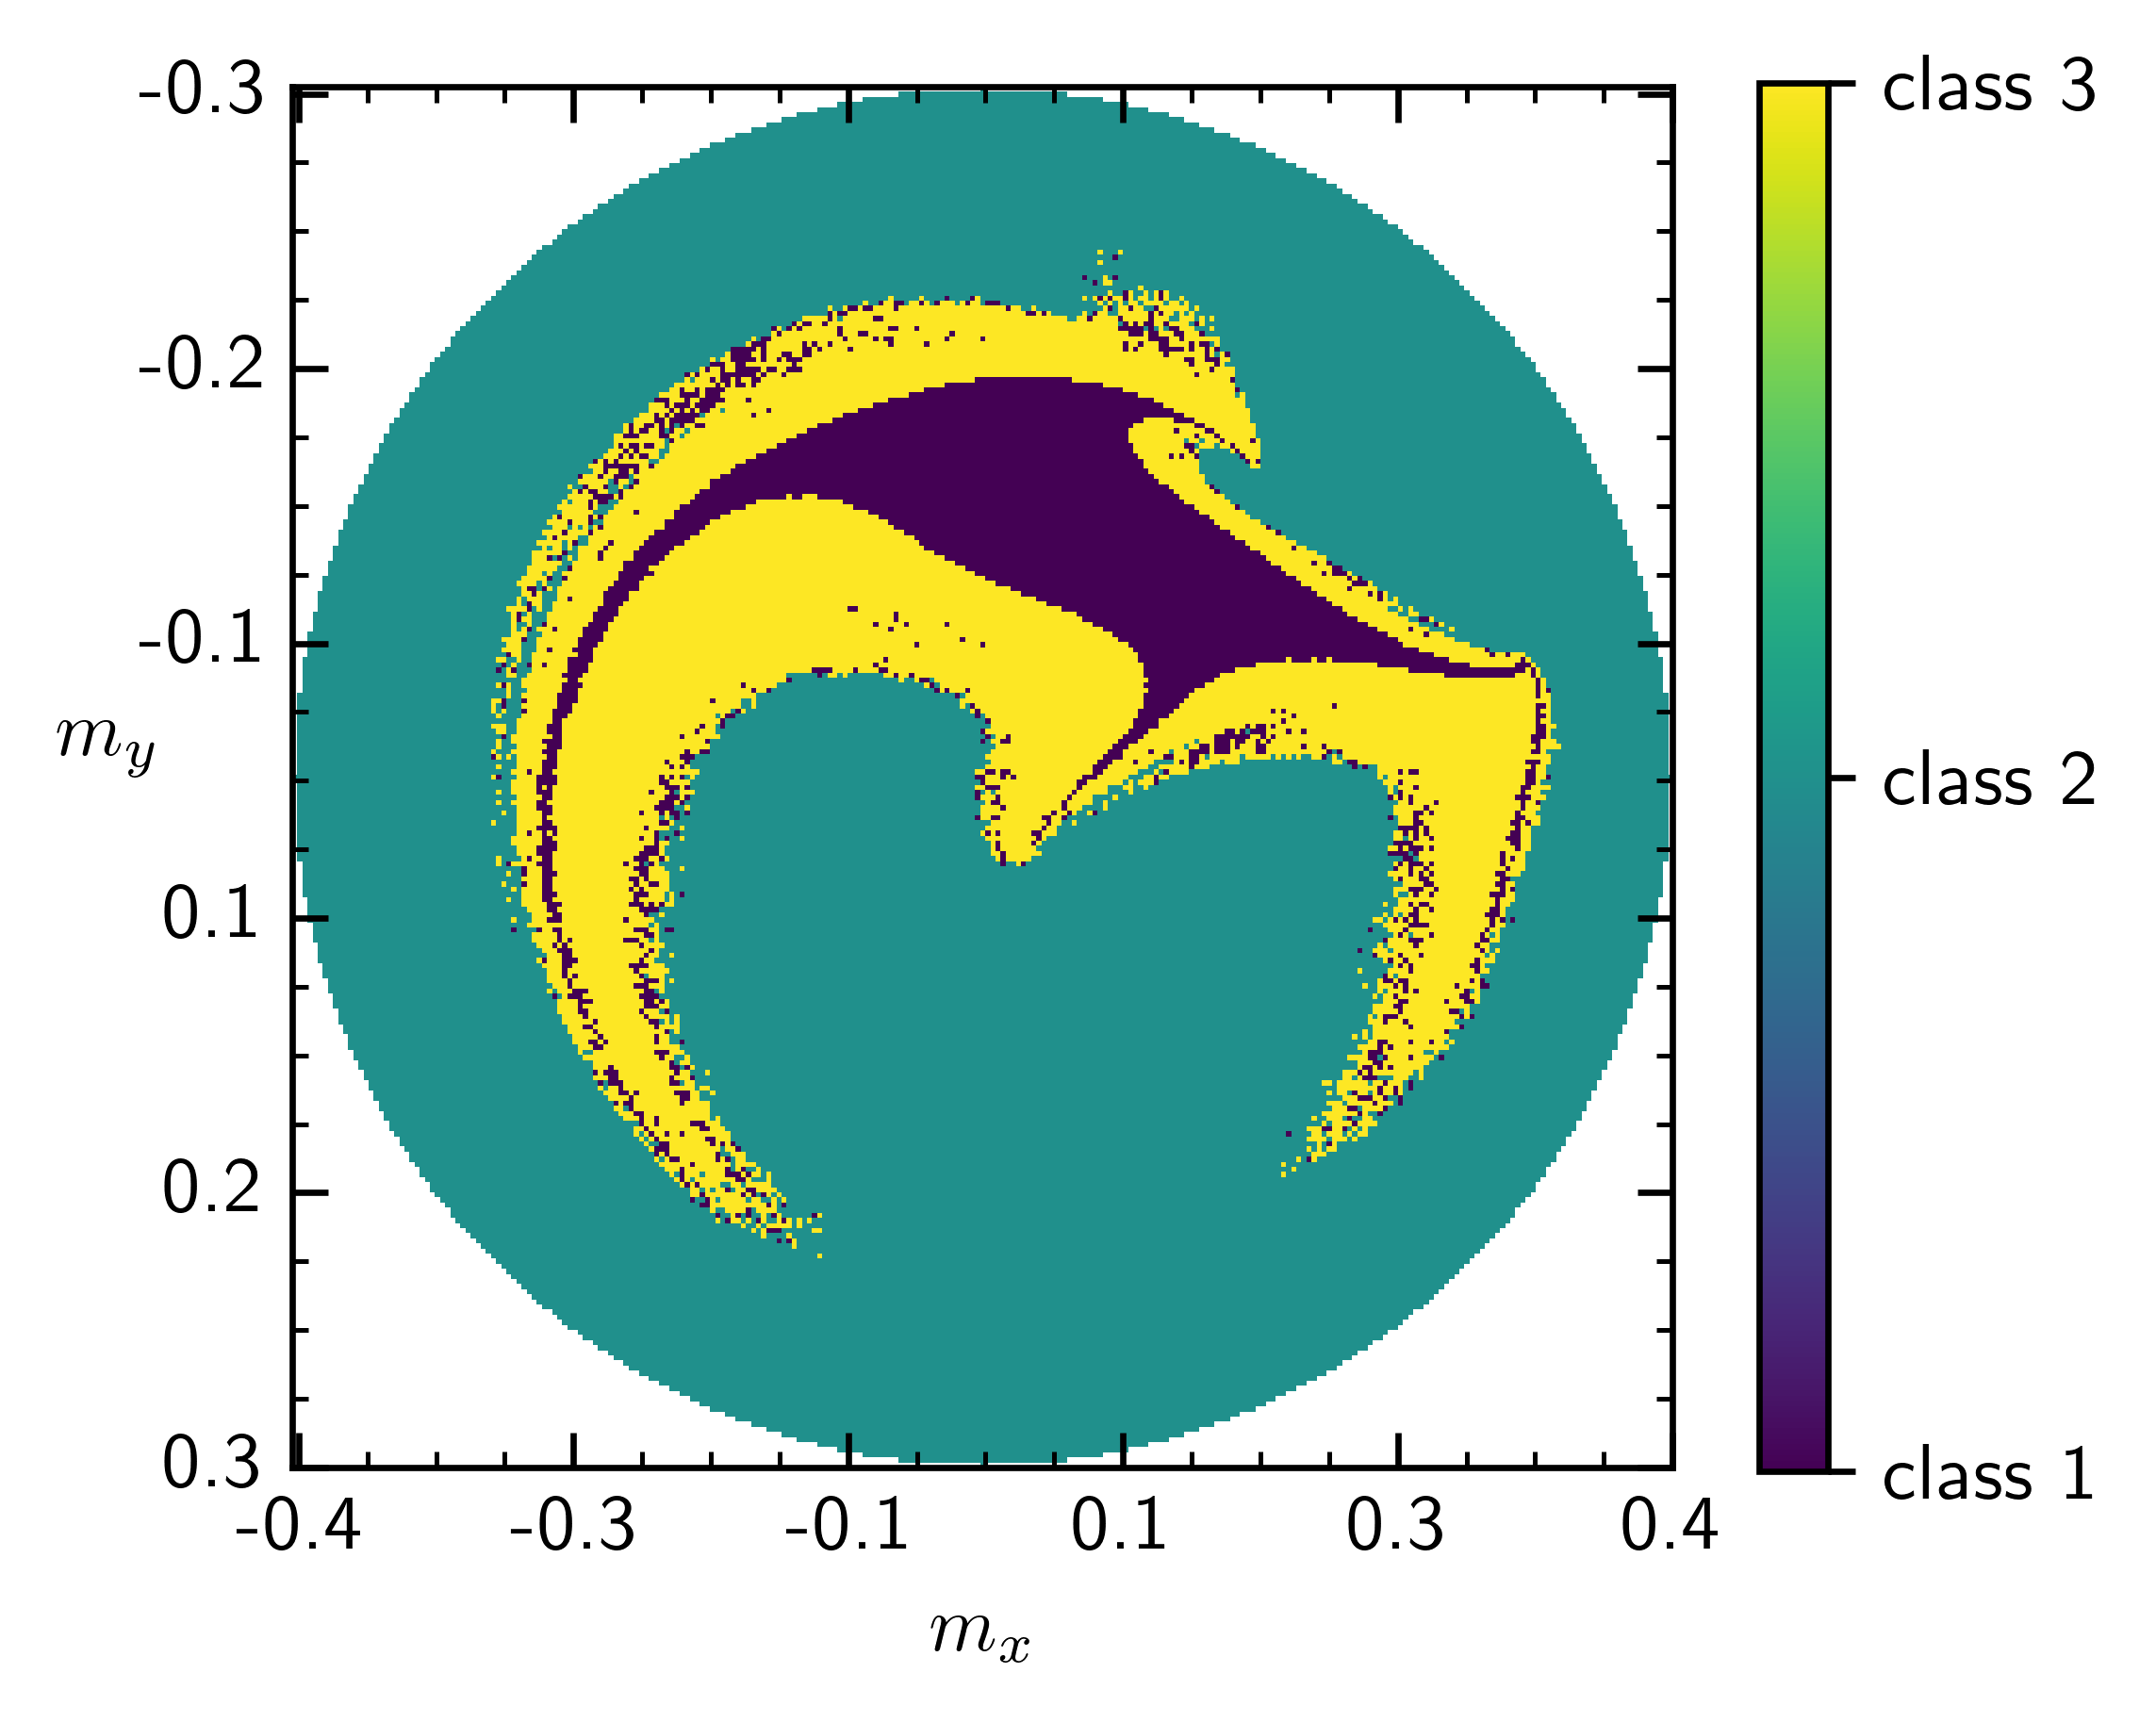
\includegraphics{pictures/phaseplot_tilted.png}
%     \caption{}
% \end{figure}
% \begin{figure}[H]
%     % \vspace*{-1cm}
%     \hspace*{-1.2cm}
%     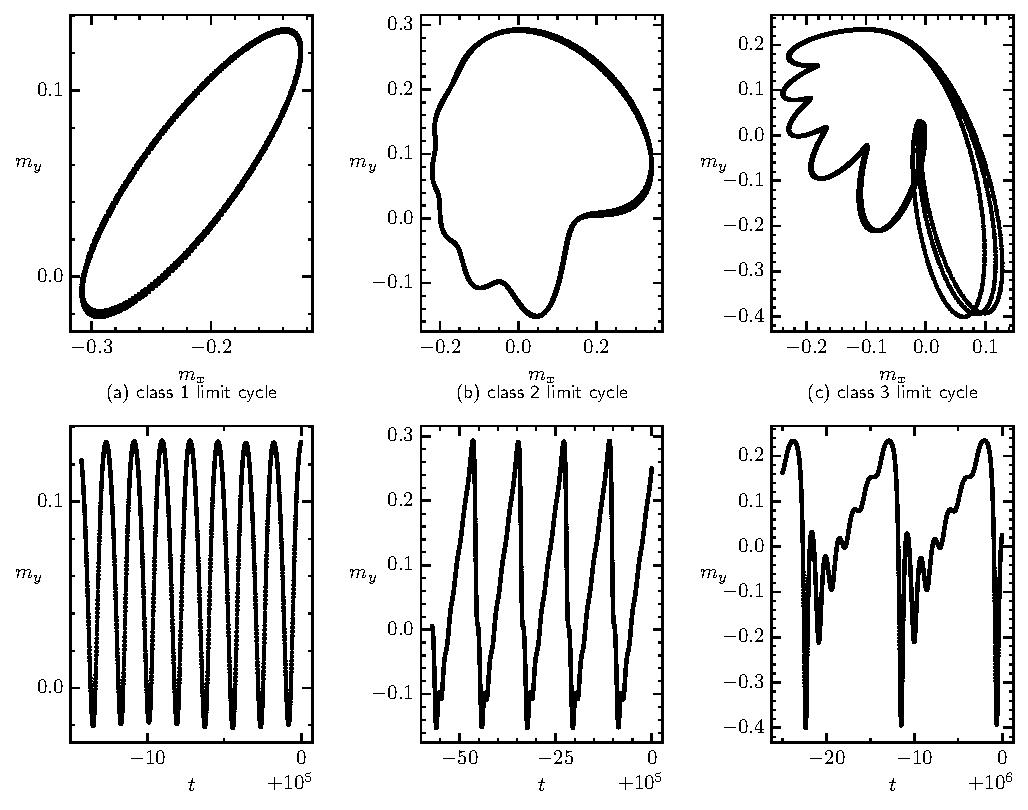
\includegraphics{pictures/classes_plot_wcut.pdf}
%     \caption{}
% \end{figure}
